\documentclass[11pt, abstracton, twoside, titlepage=true]{scrartcl}
\usepackage{a4, fullpage}
\usepackage[usenames,dvipsnames]{color, xcolor}
\usepackage{listings, caption, graphicx}
\usepackage{multicol, titlesec}
\usepackage{fancyvrb}
\usepackage{enumitem}
\usepackage{amsmath, amssymb}
\usepackage{afterpage}
\usepackage{lipsum}
\usepackage[automark]{scrpage2}

\pagestyle{scrheadings}
\clearscrheadfoot
\setheadsepline{0.5pt}

\ihead{\headmark}{}
\ofoot[\pagemark]{\pagemark}

\titleformat
	{\paragraph}
	{\normalfont\normalsize\bfseries}
	{\theparagraph}{0.5em}{}
\titlespacing*
	{\paragraph}
	{0pt}
	{1ex plus 0.5ex minus .2ex}
	{1ex plus .2ex}

\renewcommand{\lstlistingname}{Snippet}
\renewcommand{\titlehead}{\textbf}

\DeclareGraphicsExtensions{.pdf,.png,.jpg}
\DeclareCaptionFont{white}{\color{white}}
\DeclareCaptionFormat{myformat}{#1#2#3\hrulefill}

\captionsetup{format=myformat}
\captionsetup[lstlisting]{
	position = bottom,
	format = myformat
}

\lstset{
	basicstyle   = \ttfamily\color{black}	
}

\lstdefinestyle{sonicpi}{
	language = ruby,
	basicstyle   = \ttfamily\color{black},
	keywordstyle = \ttfamily\color{blue},
	morekeywords = {
		define, load_samples, each
	},
	morekeywords = {[2]{
		play, sleep, cue, sync,
		release, sample, choose, use_synth, cutoff, rrand, chord,
		ring, scale, puts, use_synth_defaults, amp, attack,
		sustain, note, octave, mod_phase, mod_invert_wave, mod_range,
		rate
	}},
	morekeywords = {[3]{
		in_thread, live_loop, loop, times
	}},
	keywordstyle = {[2]{\color{magenta}}},
	keywordstyle = {[3]{\color{ForestGreen}}},
	commentstyle = \ttfamily\color{Gray},
	stringstyle  = \color{orange}
}

\newenvironment{myitemize}{ 
\begin{itemize}
    \setlength{\itemsep}{1pt}
    \setlength{\parskip}{0pt}
    \setlength{\parsep}{0pt}     
}{ 
\end{itemize}                  
}

\newenvironment{blockquote}{
	\par
	\medskip
	\leftskip=4em\rightskip=3em
	\noindent\ignorespaces
}{
	\par\medskip
}

\def\therefore{
	\leavevmode
	\lower0.4ex\hbox{$\cdot$}
	\kern-.5em\raise0.7ex\hbox{$\cdot$}
	\kern-0.55em\lower0.4ex\hbox{$\cdot$}
	\thinspace
}

\lstset{
  mathescape,         
  literate={->}{$\rightarrow$}{2}
           {ε}{$\varepsilon$}{1}
}

\setlength{\headsep}{0.5in}
\setlength{\parskip}{0.4cm}
\setlength{\parindent}{0cm}

\let\endtitlepage\relax

\begin{document}

\subject{{\large Department of Computing \\ Imperial College London} \\
\LARGE{Individual MEng Project}}
\title{Musical Concurrent Programming \\ With Sonic Pi}
\author{{\LARGE Eleanor Vincent} \\ {\large Supervisor: Nobuko Yoshida}}
\date{\today} 

\maketitle{\thispagestyle{empty}}

\begin{center} 
	
\includegraphics[width=0.50\textwidth]{images/crest.jpg}
\end{center}

\afterpage{\thispagestyle{empty}\null\newpage}
\newpage

\thispagestyle{empty}
\begin{abstract}
We are entering into an age of computing where concurrency and 
distribution have become some of the most pressing issues in need of address. 
As we continue to outstrip the hardware of our machines, with the increased rate 
of data that we process, parallelism and exploiting concurrency are the key method
for us to handle this. An active field of theory for this is Session Types. With
session types we can model the communication protols of a program much more 
intuitively than is currently possible.

The popularity of `live coding' is also continuing to grow. With the use of 
programming centered on interactive improvisation it becomes crucial to improve 
the nature of timing within the program. Timing constraints have vast implications 
on the field of `real-time computing' where high-performance is important. By 
mimicing the understood notion of a `type-system' and developing a formalised 
idea of a `time-system' we can use to verify the timing structure of our programs.

This report describes the improvements made to the existing Sonic Pi language; a 
musical live coding language designed for educational use as a first language. We 
develop existing ideas of a formal specification for the temporal behaviour of 
Sonic Pi and present the implementation of this timing system. Alongside this 
we apply the field of session types to the underlying communication structure of 
Sonic Pi, formalise its ideas, and present the implementation of this typing 
system. By running the systematic testing suite we have designed, we prove the 
correctness of our analysis of the program against these two formalisations and 
also comment on the overall performance of the additions. We are also careful to 
review our success in presenting the information collected in a manner that 
complements Sonic Pi's construction as a first programming language. Whilst some 
features lend themselves to personal explorations, many of the timing effects 
implemented here lend themselves to the purpose of educating young people on the 
realms of concurrency and temporal reasoning.
\end{abstract}
\afterpage{\thispagestyle{empty}\null\newpage}
\newpage

\renewcommand{\abstractname}{Acknowledgements}

\thispagestyle{empty}
\begin{abstract}
\noindent\lipsum[1]
\end{abstract}
\afterpage{\thispagestyle{empty}\null\newpage}
\newpage

\thispagestyle{empty}
\tableofcontents
\newpage

\section{Introduction}
\thispagestyle{empty}

\subsection{Motivation}
% need more on the concurrency verification motivation!!
% easy to feed into how difficult that can be to teach?
For many years it has not been a requirement that children should learn much
about the vast field of computing during their formative years in UK 
Education. In 2012, the Government began to re-recognise the signifiance of 
Computer Science, after the last Cirriculum Project had been shut down in 1991, 
and has replaced the National ICT curriculum with a revised 
Computing cirruculum. The new Computing Program of Study \cite{DfE13} aims to 
enable pupils to understand the world of computing, giving them the ability to 
think logically and apply the fundamental principles of the discpline to their 
real-world environments.

The movement is not purely restricted to the UK. In the US there is a similar 
campaign calling to recognise the topic as relevant to all contempary 
sciences. It calls ``Computational Thinking'' a universally applicable 
attitude and skill set everyone, not just computer scientists, would be eager 
to learn and use \cite{Wing06}. A recent Microsoft article, as part of the 
\#WeSpeakCode campaign, claims that 75\% of students in the Asia Pacific region
wish that programming could be offered as a core subject in their schools \cite{micro}.

There is a general struggle within the humanities courses available in UK schools 
to remain relevant in light of a quickly developing technical world. Music schemes 
within the UK frequently report having suffered funding cuts and education is 
focused on learning a variety of specific instruments, with little focus on 
musical technology.

As well as recognising Computer Science and Music within schools, there 
is an increasing recognition of the power of programming amongst other disciplines. 
A growing hacker and maker movement has been making programming a 
much more accessible skill \cite{BAD14}; it presents itself as a viable and 
useful hobby amongst a vast range of ages and professions and this is as much 
because of the availability of useful resources that would be frequently used 
in such situations as a school classroom. Existing research has examined the 
viability of programming tools for professional artists, as reported at PPIG 
\cite{Ch12,BC05}, and the craft practices of existing professional software
developers who work in professional art contexts \cite{W10}.

At the same time as this we have entered an age where concurrency and 
distribution have become some of the most pressing issues in computing. As we 
begin to process hugely increased amounts of data the ideas of parallelism and 
exploiting concurrency are becoming more and more pronounced. In this day and age
it is almost impossible to find a person who does not own a mobile, most likely a 
`smart' device, which relies on communication with other such devices to function 
effectively. 

Concurrency theory has been an active field of research since the 1960s, producing
many formalisms over that time which have improved the field of computing. One 
such formalism is that of process calculi, a field that $\pi$-calculus is a strong
member of. Another type of process calculi, CSP, was highly influential in 
bringing to light such languages as Go: a relatively young language but praised
for its concurrency primitives and performance. Golang can be found in the backend
of many notable technology companies. Models of concurrency are being used for
reasoning and specification as well as at all stages of the development life
cycle: design, implementation, testing, etc...

Whilst there has been much in the field to support a programmer as they produce
type-safe code, the same cannot be said for communication-safe code. Concurrency
bugs such as deadlocks and thrashing behaviour can be as hard to locate now as
ever before. Some tools and techniques exist to handle these situations, such as
mutexes and locks \cite{T95}, but even with such tools there is no garauntee
that some obscure situation will not arise to break it on the same level as 
\emph{type-safety}.

% This is not so much a motivation - switch out for concurrency
% Sonic Pi is one of many projects designed to support both computing and music 
% lessons within schools. Sonic Pi is an environment for creating live-coded 
% music at a level of complexity which is well suited to a first-programming 
% language \cite{sp}. Many available languages are suitable as a first-programming 
% language, but not all attempt to make themselves an inviting gateway into the 
% realm of technical programming and innovation. Sonic Pi seeks to provide an 
% exploratory and invigorating introduction into programming whilst being complex 
% enough to lead a user through into much more complicated programming ideas and 
% use cases with a managable learning curve. By presenting a musical system it 
% seeks to break down the barrier between the technical elite and the hobbyist. In 
% this report Sonic Pi will be presented in terms of the formalisation of its 
% timing effects and the existing concurrency primitives of the language. 

\subsection{Objectives}
In the current version of Sonic Pi there is no means to verify the timing effects
or the communication patterns of the program. This is to say, users must judge
themselves how long the current program is, that the program is timed correctly,
and that the program is free from concurrency bugs. This can be difficult enough 
in a static environment; in Sonic Pi there is the additional requirement to do 
all of these things during a live performance (studio audience included)! The 
first point can be difficult for novice programmers, potentially moreso for 
those with little musical experience. The latter can be difficult for even some 
experienced programmers due to the non-deterministic nature of some concurrency 
bugs.

In building analysis for the timing effects of the program, we hope to develop
something that is sufficiently lightweight so that it may be run during a live 
performance of the program. This leads to interesting challenges in terms of the 
heuristics used when parsing the program and what solutions will lead to the best 
possible results. We plan to utilise the speed of the platform and program 
architecture and efficient design for this matter.

In developing the communication patterns of Sonic Pi we aim to utilise the
theory of Session Types and apply them to this context. Session Types will
enable us to define a clearly understandable structure to the communication
protocol of the program; this will enable the tool to identify difficult bugs
such as deadlocks and thrashing behaviour. In identify problems in this manner,
we will be able to reduce the number of crashes developers experience whilst 
writing code `on-the-fly'.

\subsection{Contributions}
We have produced a lightweight shared library, often affectionately referred to 
as Sonic-Verify, that enables a variety of different analysis of a program 
written for the Sonic Pi IDE. The project analyses the timing effects of the 
program, outputting such information as the total `virtual time' elapsed by the 
program and more specific detail, such as function durations. This implementation
of a formal timing system presents an improved environment in which developers
may code more asthetically pleasing music in a live environment. 

This is also the first instance of the theory of Session Types being applied in 
a (musical) live programming context. With this analysis we are able to output 
the decomposed types of all processes in the program and the associated global 
type, presenting an intuitive description of the interactions of processes 
within the source code. This presents an exciting new realm of possibility in
terms of concurrency verification and the application of Session Types in 
existing distributed paradigms.

We have implemented a set of tests that systematically verifies the results that
our project produces; it covers a range of features starting from the most basic
of sequential programs through into full music sources, with complex function
call structures and multiple interacting process threads. Finally, we have fitted
this library into the existing Sonic Pi IDE in a manner that is beneficial to both
new coders and `old hat's alike. 

\subsection{Report Structure}
The remainder of this report is broken down as follows:

\begin{itemize}
	\item Background: We detail the basic concepts of Sonic Pi and its timing 
	effects, and Session Types to give an adequate foundation for the work 
	presented in this project. We also explore the field of Live Programming 
	as part of the background research.
	\item Related Work: We detail the existing work in the field Live Programming
	with a particular focus on those with musical contexts. We also detail some
	of the existing applications of Session Types, outlining the approaches and
	differences therein.
	\item Design \& Technical Implementation: Here the chapter is broken into
	two core sections, focusing on both the timing effects of Sonic Pi and
	the session types of Sonic Pi in turn. We discuss chosen languages and key
	libraries used in the design of the program and then move into general
	implementation and interesting algorithms and code from each section. The
	section concludes with a brief discussion of the architecure of the Sonic 
	Pi IDE and how we chose to integrate our verification library.
	\item Evaluation: Here we evaluate the success of the project. We discuss
	the limitations of the current state of the project and outline qualitive
	and quantative metrics for the project, including a systematic test of
	the correctness of our approach.
	\item Conclusion: Here we present possible improvement for the project in
	the future work section before closing with a summary of those objectives
	achieved.
\end{itemize}
\newpage

\section{Background}
\thispagestyle{empty}
In this section we begin with a short history of Computing in Schools followed 
by explaining the ideas and features of Sonic Pi, the live coding IDE that forms 
the basis of this project. We then move on to explain the subject of both Live 
Programming and Session Types in further detail and seek to relate them back to 
the current aims of the project.

\subsection{Computing in Schools}
Some of the earliest significant pieces of work towards the 
education of computing started with the invention of Logo, an adaptation of 
the LISP language, most remembered for its use of ``turtle graphics''. Some 
time after this came the Computers in the Cirriculum Project, funded from 
1972 to 1991 by the Schools Council with addition aid from the Microelectronics 
Education Programme introduced in 1981. The first microcomputers appeared in 
both UK Primary and Secondary Schools in 1979. The Commodore Pets aided both 
spelling and arthimetic practice as well as the ability to teach either BASIC or 
Logo. The 1980's saw a huge amount of legislative reform and technical efforts 
to give young people the ability to work with computers. Unfortunately, over the 
course of the late 80's and early 90's, this focus on programming ability gave 
way to simply the education of practical use of existing computer software; 
there was little to no focus on the programming fundamentals behind 
these applications \cite{naec}.

In 2013, Ofsted published a report documenting their findings relating to ICT 
in UK schools from 2008 to 2011 and found that in half of all secondary 
schools, school leavers had not been given adequete education to move into a 
technical career in their future. In 2007, 81,100 pupils were enrolled in the 
ICT GCSE but this had fallen to 31,800 pupils by 2011 \cite{DfEO13} with a 
notable lack in the education of key skills such as computer programming 
itself. This lack was found to be as much a lack in knowledge from the 
teacher's as much as the cirriculum's failure to address the issues.

\subsection{Sonic Pi}
Sonic Pi is an imperative live programming language designed as an educational 
first language. It is a Ruby-based Domain-Specific Language designed for 
manipulation of synthesisers through time \cite{AB13}. It is interpreted through 
a VM rather than being directly compiled. It is currently in its 
second iteration, with the main extension between the two languages being the 
work done to improve the timing system of the project, which is discussed in 
more detail below. Sonic Pi is built on top of the SuperCollider synthesis 
server to enable it to define and manipulate synthesisers in real time; an 
important feature for a musical language. Some of the concepts that Sonic Pi 
is well suited to teach, in direct relevance to the current UK Computing in 
Schools Cirruculum, are conditionals, iteration, variables, functions, 
algorithms and data structures. Sonic Pi also extends beyond these concepts to 
include such features as multi-threading and hot-swapping of code as these are 
likely to be of crucial importance in the future of programming contexts \cite{
AOB14}. It also presents an inviting environment to teach concepts such as 
parallelism and concurrency; a core strength of the program as these can be
notoriously difficult concepts to explain.

This section first gives a brief description of the Raspberry Pi then explores 
the implementation of Sonic Pi V1.0, mainly to give appropriate context to the 
timing system that Sonic Pi V2.0 currently imeplments. There is then a 
short discussion on the features of Sonic Pi V2.0.

\subsubsection{Raspberry Pi}
The Raspberry Pi was developed as a very low cost computer system to enable 
technical experimentation amongst people who have little access to computers 
they could tinker with or expose the programming layer. The idea came about in 
2006 as an answer to the steadily decreasing levels of pupils applying to take 
up Computer Science after their A-Levels. The reasons for this were attributed 
to many contributing events such as the end of the ``dot com'' boom, the focus 
of IT lessons on Microsoft software and building very basic HTML websites and 
the increased availability of out-of-the-box games consoles over the Amiga, BBC 
Micro, Spectrum ZX and Commodore 64 machines that promoted individual 
experimentation so freely in the past \cite{rp}.

The Pi is provided as a bare circuit board costing roughly \$25, able to boot 
into a Linux environment with very little other commerical equipment required. 
The Raspberry Pi Foundation is a non-profit organisation and has sold over a 
million products since 2012. The main objective is to develop genuine 
technical competency by allowing the freedom to experiment with the whole 
system rather than taking the locked box approach of other systems. Learning 
becomes self directed for pleasure rather than at the behest of a mark molded 
system. It is this style of engagement that brought the Raspberry Pi to the 
attention of educational campaigners and has since enabled it to be used so 
successfully within the new movement towards better Computing education within 
Schools. 

\subsubsection{Sonic Pi V1.0}

\begin{multicols}{2}
Sonic Pi V1.0 was designed to port the language Overtone to the Raspberry Pi in 
order to focus on driving specific educational objectives; the idea in mind was 
to teach a target audience of 12-year-olds that had no previous experience with 
programming; it would bring them from the state of ``this is a computer'' through 
to the ability to write a full length program, that generated satisfying music, 
over the course of a few weeks. Sonic Pi is a Ruby-based language both due to 
the author's existing experience with the language and to keep it in line with 
the languages already used within the industry. Python is well regarded as an 
education language and the semantic similarity between the two makes Ruby easy 
to defend as a language choice.
\\

\begin{minipage}{0.5\textwidth}
	\begin{minipage}[t]{\textwidth}
		\begin{lstlisting}[style = sonicpi]
	play 60
	play 61
	play 62
		\end{lstlisting}
		\captionof{lstlisting}{Chord Form: Successive Notes}
	\end{minipage}

	\begin{minipage}[t]{\textwidth}
		\begin{lstlisting}[style = sonicpi]
	play 60
	sleep 0.5
	play 61
	sleep 0.5
	play 62
		\end{lstlisting}
		\captionof{lstlisting}{Arpeggio Form: Sleep Separation}
	\end{minipage}
\end{minipage}

\end{multicols}

The immediate feature that Sonic Pi focuses on is sequential ordering in 
imperative programs; demonstrated in musical theory by the sequential playing 
of notes. Code Snippets 1 and 2 demonstrate two small Sonic Pi programs. The 
first demonstrates the situation where the MIDI notes would be played together. 
Sonic Pi v1.0 takes advantage of fast clockspeeds of modern processors in order 
to assume the sequence of instructions would execute quickly enough 
to sounds together. In order to separate them into sequential notes they must 
be separated with a sleep instruction as demonstrated by Snippet 2. The notation 
for sleep in Sonic Pi V1.0 is similar to that of the POSIX sleep operation 
\cite{IG13}. The default sound that Sonic Pi uses in these contexts is a 
pleasant bell sound from the SuperCollider synthesiers.

It can be seen that the ability to skip the arguably verbose nature of 
structured syntax makes it much more relevant in the contexts of a classroom; 
pupils are able to start creating meaningful programs with much more speed. From 
the point of view of providing any future debugging interfaces, it has a small 
benefit in removing the code overhead for finding and correcting such small 
syntactical issue such as missing \texttt{;}. 

These semantics work well in an educational context but do not allow for the 
correct timing of musical notation which puts them at odds with user 
expectations. To demonstrate this more concretely, below are two further code 
snippets demonstrating Sonic Pi's basic threading abilities. Sampling is a 
feature of Sonic Pi V2.0 but is presented here in the context of V1.0 
programs as the two versions are syntactically similar.

\begin{multicols}{2}
In Snippet 3 the desired outcome is to play MIDI note 60 together with the 
drum kick with an interval of 0.5s between each hit. Unfortunately, this does 
not take into account the execution time of each statement; there is a short 
amount of execution time for each line of code, plus the desired sleep of 0.5s.
Because of this the rhythm will gradually shift with each loop as the 
clock time and the ``virtual time'' becomes further out of sync. The 
actually length of time each line execution takes is variable between 
processors depending on their speed and overall load. Regardless, we can see 
that each loop in Snippet 3 will actually take longer than the desired 0.5s.

This is further apparent when running Snippet 4. The desired outcome is to 
play the drum kick every second and the MIDI 60 note at every half second, so 
the two notes will play at the same time every second MIDI note, the threads 
remain synchronised. On running the threads it is quickly apparent that this 
is not the true result; due to differing execution times the thread rhythms 
drift apart very quickly.

	\begin{minipage}{0.5\textwidth}

		\begin{minipage}{\textwidth}
			\begin{lstlisting}[style = sonicpi]
loop do
    play 60
    sample :drum_heavy_kick
    sleep 0.5
end
			\end{lstlisting}
			\captionof{lstlisting}{Repeating Bass and Drum}
		\end{minipage}

		\begin{minipage}{\textwidth}
			\begin{lstlisting}[style = sonicpi]
in_thread
    loop do
        play 60
        sleep 0.5
    end
end

in_thread
    loop do
        sample :drum_heavy_kick
        sleep 1
    end
end
			\end{lstlisting}
			\captionof{lstlisting}{Concurrent Threads}
		\end{minipage}

	\end{minipage}

\end{multicols}

The $play$ and $sample$ calls are asynchronous and this compounds the present 
timing issue due to additional costs in sending and interpreting the messages. 
These issues are summarised in Figure 1. The left-most column represents the 
real computation time of the statement whilst the right-most column shows the 
point at which each statement would be run. Each statement duration is unique 
as processor speed and system load variations affect the duration of each 
statement separately. The durations are therefor non-deterministic in nature 
and also not consistent across different runs of the same program.

\begin{figure}[ht]
	\centering
	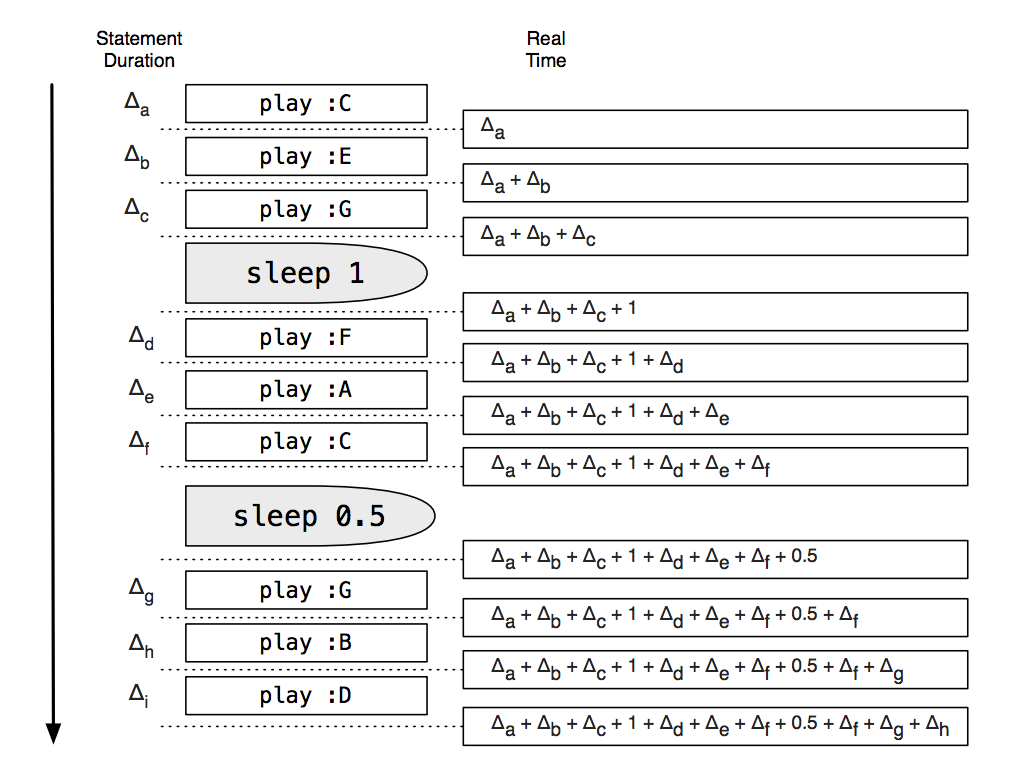
\includegraphics[width=0.9\textwidth]{images/sonic-one.png}
	\caption{Timing in Sonic Pi V1.0 \cite{AOB14}}
\end{figure}


\subsubsection{Sonic Pi V2.0}

\paragraph{Timing Sleep}
Sonic Pi V2.0 sought to address this temporal issue and introduces the 
interesting concept of a \emph{time system} and associated \emph{time safety}, 
which draw an analogy from the familiar programming concepts of \emph{type 
systems} and \emph{type safety}. V2.0 maintains syntactic 
compatability with V1.0, so it as conceptually useful to apply in the 
educational context as before. The power behind V2.0 is that its temporal 
semantics now react as a user would expect them to, making it a viable program 
for the musically experienced who have some concept of what they want to 
achieve as well as for those beginners who desire to learn.

In Sonic Pi V2.0 the sleep command no longer mimics the POSIX command as 
commented earlier. Instead the programming model allows a separation of the 
ordering of effects from the timing of effects. Snippet 5 shows a simple 
example that combines the different kind of effects; parallel, timed and 
ordered effects. It also demonstrates further syntactic abilities of V2.0 as 
we are now treating the code snippets as V2.0 programs.

\begin{minipage}{\textwidth}
	\begin{lstlisting}[style = sonicpi]
		  play :C ; play :E ; play :G
		  sleep 1
		  play :F ; play :A ; play :C
		  sleep 0.5
		  play :G ; play :B ; play :D
	\end{lstlisting}
	\captionof{lstlisting}{V2.0 Program: Playing three chords (C major, F major, G major)}
\end{minipage}

Each chord line demonstrates Sonic Pi's ability to play notes in parallel, the 
system still taking advantage of the capabilities of modern processors. \texttt
{sleep} now acts as a ``temporal barrier'' between statements; it works by 
blocking computation from proceeding until the given time has elapsed \emph{
since the program began running}. It does \emph{not} block from the end of the 
notes played. In terms of Snippet 5, this means that the second chord is 
played once one second has elapsed and the third chord will not be played 
until 1.5 seconds have elapsed. One can think of \texttt{sleep} as an ``at 
least'' timing. In other words, once \texttt{sleep t} has been evaluated, we 
can state that at least \texttt{t} seconds have elapsed since the last \texttt{
sleep} statement was called. This is similar to how the language ChucK handles 
the interaction of time using its (multiply) overloaded \texttt{=>} operator 
\cite{WC03}.

For completeness it is worth noting that Snippet 5 demonstrates the ordered 
effect as the three chords are played in the order written.

\begin{figure}[ht]
	\centering
	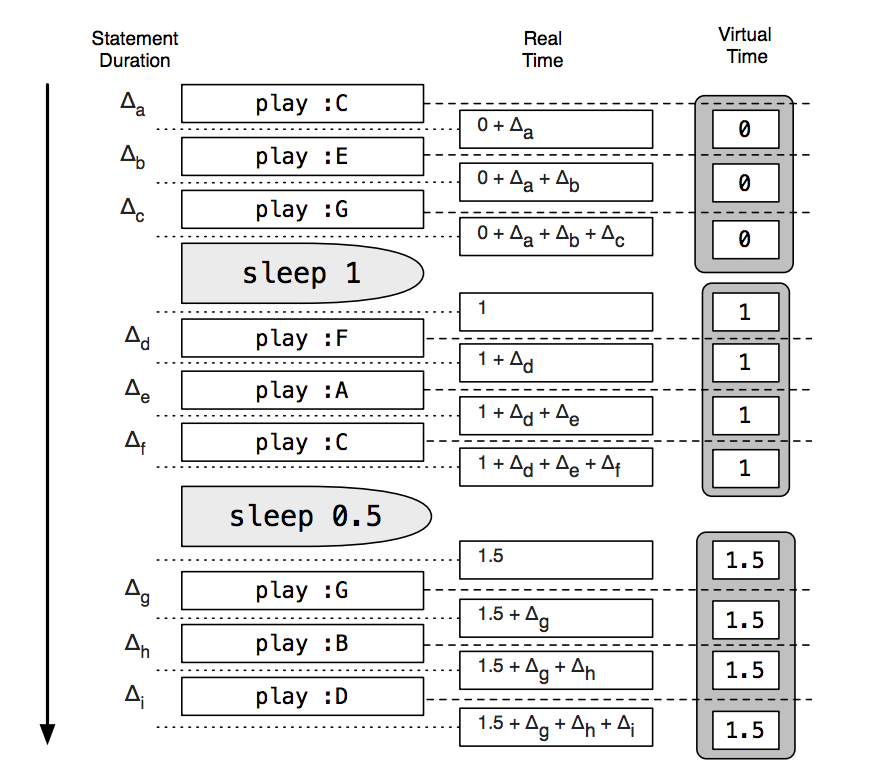
\includegraphics[width=0.8\textwidth]{images/sonic-two.png}
	\caption{Timing in Sonic Pi V2.0 \cite{AOB14}}
\end{figure}

The semantics introduced here are achieved by implementing the concept of 
``virtual time''. In Sonic Pi V2.0, virtual time is a 
thread-local variable that is only advanced by a new \texttt{sleep} command, 
which means that the programmer has explicit control over the timing of the 
program. Each thread maintains access to both the real time elapsed and the 
virtual time elapsed whilst running a given program and used the virtual time 
variable to scheduled requested effects. In order to keep time with the 
explicit timing requirements of the program the \texttt{sleep} command will 
take account of the execution time between the last \texttt{sleep} statement 
and the current execution point. Referring back to Snippet 5, at the point at 
which the program executes the second \texttt{sleep} command, if execution 
of the F major chord took 0.1s of execution time then the program will only 
sleep for 0.4s. This is to ensure there is no rhythm drift; the only overhead 
in the rhythm is from the play statements following the last \texttt{sleep} 
executed. This is demonstrated visually with Figure 2.

To deal with the non-deterministic execution times within a sleep barrier, and 
also to deal with the time cost for the synthesiser to schedule output 
effects, a constant \texttt{scheduleAheadTime} value is added to the current 
virtual time for all asynchronously scheduled effects. If the 
execution time between \texttt{sleep} commands never exceeds this value then 
the temporal requirements of Sonic Pi are met. 

It is possible that the time between \texttt{sleep} commands may over-run - 
this may be common in the event someone requested a short \texttt{sleep} time 
such as 0.1s or even 0.05s. In this case, the described programming model is 
not useful for providing hard deadlines but can function with ``soft'' 
deadlines (along the vein of Hansson and Jonsson \cite{HJ94}). In the event a 
thread falls behind in execution time then the user is given explicit 
warnings. Should the amount of time the thread is behind exceed a specific fall
-behind value, as defined within Sonic Pi, then the system will stop that 
thread and throw a time exception. This provides essential temporal 
information about the program and its behaviour to the users. This is a 
positive in terms of educational use but is something a live coder will aim to 
avoid during a real performance. This feature also provides a safety mechanism 
against common errors such as placing isolated \texttt{play} calls between 
\texttt{sleep} commands which would have the problem of taking up all of the 
system resources; instead the thread self-terminates and allows any other 
threads to continue executing.

\paragraph{Threading}

Threading has already been introduced breifly; this section focuses on the 
further improvement that Sonic Pi V2.0 brings to its threading primitive. 
Within V2.0 there are multiple commands which allow for easy synchronisation 
of threads whilst the program is running. Threads also implement thread-
based inheritance wherein they take all of the synthesiser settings of the 
thread they were spawned from.

The keyword \texttt{in\_thread} enables Sonic Pi users to run pieces of 
code concurrently. Threads can be named as shown in Snippet 6 in a similar way 
to how functions are named in Sonic Pi. The simple nature of its loop syntax 
enables this to be as easy a concept to grasp as the previously defined 
temporal semantics. These threads alone do not allow for the live coding that 
Sonic Pi has been created for; a developer must combine each thread with a loop
in order to produce constant sound. Sonic Pi V2.0 provides the \texttt{live\_loop}
keyword to capture the same effect with less writing.

An interesting point to note about Sonic Pi V2.0 is that actually running the 
program starts the current program in another thread. Because of this one can 
actually press run multiple times and have the program layered over the top of 
itself. There are no particular synchronisation primitives defined over these 
``global'' threads, but it makes for an interesting performance if timed 
correctly.

\begin{minipage}{\textwidth}
	\begin{lstlisting}[style = sonicpi]
    in_thread(name: :bass) do
        loop do
          use_synth :prophet
          play chord(:e2, :m7).choose, release: 0.6
          sleep 0.5
        end
    end

    in_thread(name: :drums) do
        loop do
          sample :elec_snare
          sleep 1
        end
    end
	\end{lstlisting}
	\captionof{lstlisting}{Named Threads}
\end{minipage}

\begin{minipage}{\textwidth}
	\begin{lstlisting}[style = sonicpi]
    live_loop :foo do
        play :c1, release: 8, cutoff: rrand(70, 130)
        sleep 8
    end
	\end{lstlisting}
	\captionof{lstlisting}{Live Loops}
\end{minipage}

While running a program, Sonic Pi's \texttt{live\_loops} will automatically update 
the program without skipping any beats. This gives the users a great amount of 
freedom to experiment with different sounds without having to reset the program
with every small edit, as is the case with standard 
programming. This feature, however, is directly affected by the previously 
described temporal semantics; loops can easily become out of time with 
each other during a performance. To combat this, Sonic Pi provides 
synchronisation semantics in the form of the \texttt{cue} and \texttt{sync} 
commands. Each time a \texttt{live\_loop} loops it will generate a new \texttt{cue} 
event which we are able to \texttt{sync} on to. \texttt{cue} is an asynchronous,
non-blocking operation and \texttt{sync} is a blocking operation.

\begin{multicols}{2}
The Snippets to the right demonstrate a rough workflow of how a user would use 
the \texttt{cue} and \texttt{sync} features. To begin with we assume the loops 
\texttt{:foo} and \texttt{:bar} are out of time.

We can start to fix the situation by 
changing the sleep time in \texttt{:foo} to 0.5s. Most likely, this will still 
sound incorrect. This is because the two loops are likely to now be out of 
time with each other. Both \texttt{:foo} and \texttt{:bar} are producing \texttt{
cue} events, but these are not being used and so both loops are running with 
no regard to the other. We can fix this by \emph{syncing} one thread to the 
other, so that it will only fire when the other thread has looped (since
a \texttt{live\_loop} will send a \texttt{cue} message at the start of each loop).
In this case we have synced \texttt{:bar} onto \texttt{:foo}'s \texttt{cue} 
message.

This gives way to some very obvious deadlock scenarios (example shown in Snippet 10) 
that users must avoid. Here we have created two \texttt{live\_loop}s, \texttt{:foo}
and \texttt{:bar}. Both threads finish with a blocking call, waiting for a
\texttt{cue} message from the other loop. The issue here is, since both loops 
are blocked at the same time, neither loop will ever trigger another \texttt{cue}. 

	\begin{minipage}{0.5\textwidth}

		\begin{minipage}{\textwidth}
			\begin{lstlisting}[style = sonicpi]
live_loop :foo do
    play :e4, release: 0.5
    sleep 0.4
end

live_loop :bar do
    sample :bd_haus
    sleep 1
end
			\end{lstlisting}
			\captionof{lstlisting}{Out of Sync Live Loops} \label{outofsync}
		\end{minipage}
		\begin{minipage}{\textwidth}
			\begin{lstlisting}[style = sonicpi]
live_loop :foo do
    play :e4, release: 0.5
    sleep 0.5
end

live_loop :bar do
    sync :foo
    sample :bd_haus
    sleep 1
end
			\end{lstlisting}
			\captionof{lstlisting}{Synced Live Loops} \label{synced}
		\end{minipage}

	\end{minipage}
\end{multicols}

\begin{minipage}{\textwidth}
	\begin{lstlisting}[style = sonicpi]
	live_loop :foo do
	    play :e4, release: 0.5
	    sleep 0.5
	    sync :bar
	end

	live_loop :bar do
	    sample :bd_haus
	    sleep 1
	    sync :foo
	end
	\end{lstlisting}
	\captionof{lstlisting}{Deadlock - both loops waiting for cue}
\end{minipage}

\paragraph{The IDE}
The IDE is as much a part of the educational experience as the language 
itself. Sonic Pi features a bespoke environment that contains only the bare 
minimum features required to enable pupils to start coding quickly and with 
minmal confusion. For this reason the IDE only consists of five key components:

\begin{itemize}
	\item Control Buttons
	\item Workspace Tabs
	\item Editor Pane
	\item Information Pane
	\item Error Pane
\end{itemize}

\begin{figure}[t]
	\centering
	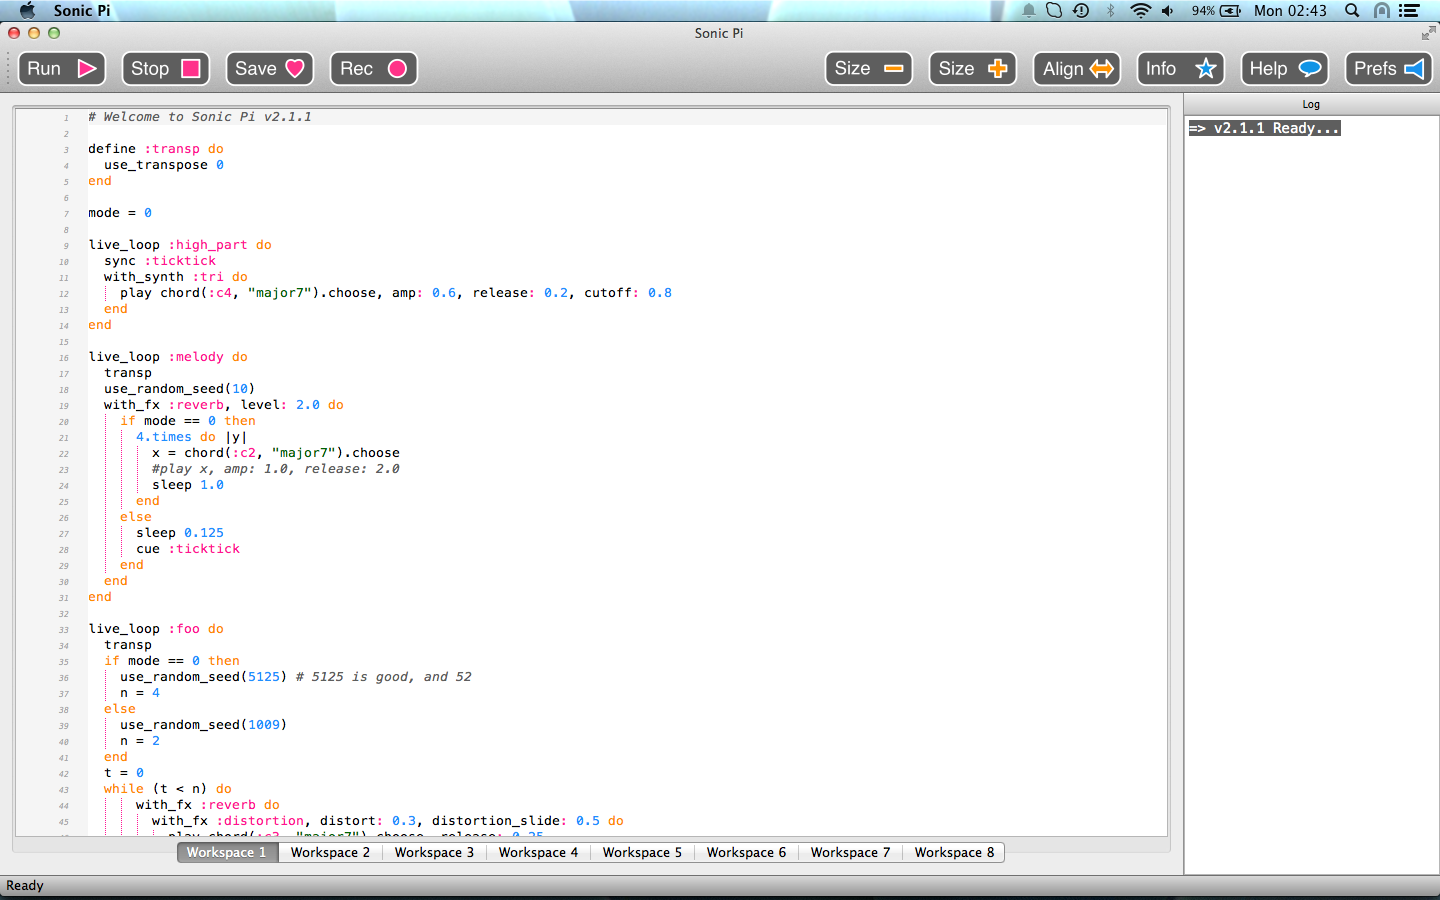
\includegraphics[width=\textwidth]{images/sonic-ide.png}
	\caption{Sonic Pi V2.1.1 IDE - Apple Mac View} \label{macview}
\end{figure}

Sonic Pi originally choose not to have a file save system as the workspaces 
automatically save the current session. There were no other usual IDE features 
such as project structure, macro system, refactoring wizard, etc... This is to 
keep the system as simple as possible to make it quick for young pupils and non
-IT teachers to get to grasps with.

Since then, in Sonic Pi V2.1.1, it has added the ability to save the current 
workspace to your file system, the ability to record what is playing and save 
as a .wav file type, basic formatting buttons, the ability to import other 
music files as custom samples, information and tutorial sections, all whilst 
remain simplistic and easily useable. Features are non-intrusive but 
incredibly useful in terms of allowing those pupils who thrive with the system 
to continue to experiment outside the scope of the regular cirruculum lessons.

\subsection{Live Programming}
For much of the prevailing history of programming there has been an idea that 
the programmer is inherently separated from the system that they are 
producing. The task of the programmer is to create a system based on some 
formal specification that will take effect at some unknown point in the 
future, and the time between implementation and action has no effect on the 
results that the system will produce. In this way, there is a strong sense of 
separation between the program, process and task domains where the progam is 
the code implementation and specifications, the process is the running of the 
code on a specific machine and the task is the visible real world results
\cite{SG10}. This is a viewpoint that many would not think to challenge as it 
is natural to assume that the methodology of a computer programmer would 
naturally lend itself to implementation of actions that were set for execution 
in the future and, in general, would process a deterministic set of results 
that can be repeatedly used as the users required.

Live programming (also referred to as With Time Programming or Just In Time 
Programming) seeks to apply the improvisional nature of time to the existing 
methodology of the programmer. With this idea it becomes possible to define a 
tigher system of feedback between the program and task domains through means 
of whatever process domain is most suitable. The improvisional nature of the 
acitity also removes the inherent requirement of a specific program 
specification and allows for new level of freedom and creativity in the 
programs being created. 

Given the nature of Live Programming the languages that invoke it are often 
dynamic languages which allow for the flexibility, conciseness and ease of 
development \cite{McD07} to enable the act of live programming to feel as 
natural as standard programming practice.

Live Programming lends itself also to acts of performance, where Live Coders 
perform to live audiences, often producing such things as live 
improvisational music or artwork, whilst having some means by which the 
audience will also see the code written at the same time. For a Live Coder 
there is frequently no desire to create a final software product or even a set 
musical score as live programming is about the experimentation rather than the 
manufacture. From a social and cultural viewpoint, Live Programming lends 
itself to breaking down the barriers that have been built up between software 
technology and the creative users \cite{McL13}.

It is interesting that the user's level as a musician will have specific 
impacts on their experience with the systems in use in the context of live 
programming and audio languages. Musical scores provide an implicit time 
representation whilst most musical languages tend to use explicit temporal 
structures. This generally makes the representation of rhythm within the 
language guarantee only the ordering of the notes and not the time elapsed 
between playing each one; the temporal structure provides no clear guarantee as 
to execution length. In terms of musical experience, non-experienced 
users may be able to identify an odd sound within this system but be unable to 
pinpoint exactly what causes the problem. 

The question of time and temporal semantics within computing has been in 
existence for some time, but live programming as a field is a very young 
research area, with most of the popular languages appearing over the last 
decade. This comes as part of a wider movement of programming reaching more of 
the general populace and as it is applied with more and more creative outlets 
in mind, this separate way of thinking about the programming environment is 
likely to produce more interesting projects as time develops. 

\subsection{Session Types}
Over recent years there has been a massive increase in the amount of 
communication based systems, from network protocols over the Internet to server
-client systems in local area networks to distributed applications on a global 
scale. The crucial observation amongst all of these systems is that while 
there may be some way to describe a one-time interaction between processes 
there is no real construct to structure a series of reciprocal interactions 
between two parties \cite{HVM98}.

Session Types present a solution to the issue of structing communication-based 
software. In a similar way to how Object Oriented paradigms sought to solve 
the issues presented by large scale system written largely with spaghetti 
code, Session Types seek to restructure existing complex behaviours in a 
manner which is more lucid, readible and ultimately more easy to verify. Honda 
et al \cite{HVM98} present this in terms of simple concurrent primitives that 
build up a basic structuring method for communication-based concurrent 
programming. In terms of this project, we will initially be using simple 
communication primitives to check the program for such concurrency bugs as 
deadlocks. Sonic Pi appears a simple language to apply the theory of Session 
Types to but the dynamic and concurrent nature of the language give it some 
interesting communication patterns to formalise. Session Types 
are also designed in a language agnostic manner, meaning it will be possible to 
apply to Sonic Pi's Ruby-like syntax.

Session Types consist of the following key ideas:

\begin{itemize}
	\item A basic structural concept known as \emph{sessions}. These are designated 
	via \emph{channels}. The collection of session interactions is what constitutes a 
	program; those interactions are performed via the channels. As well as the 
	session, other concurrent programming contructs are provided: parallel 
	composition, name hiding, conditional and recursion. The combination of 
	recursion and sessions allow for the expression of an unbounded thread of 
	interaction as a single abstraction unit.

	\item Three basic communication primitives that all other structures will be 
	built from: \emph{value passing} - standard synchronised message-passing, 
	\emph{label branching} - purified method invocation, devoid of value passing - and 
	\emph{delgation} - the passing of a channel to another process. Alongside 
	sessions, these allow for complex communication structures to be defined and 
	described with clarity.

% flesh out detail and remark that the theory is not outlined here as
% there is no focus on the implementation of this in this project
% it would be good to extend the project to include a formal typing system
	\item Finally there is a basic type discipline for the communication primitives. 
	Without this there would be no way to guarantee the typability of a program, 
	ensuring that two communicating processes always have compatible patterns of 
	communication. It is the incompatibility of interaction patterns that is one 
	of the main reasons for bugs in commmunication-based programming\footnote{We choose not to present the full formalisation of the type system 
	in this report as the focus is much more on the construction of the 
	communication protocols than on their underlying types. Interested parties can 
	read on this futher in such papers as \cite{HVM98} and \cite{HYC08}}.
\end{itemize}

\subsubsection{Multi-Party Session Types}
Multi-Party Asynchronous Session Types are a class of behavourial types
specifically targeted at describing protocols in distribute systems
based on asynchrounous communication\cite{CCPY15}. As described previously,
communication interactions are intended to occur within the scope of many
private channels following strict protocols which we have labelled as
\emph{sessions}. In it's simplest form this takes place between just two
peers, hence our previous focus on ``binary'' session types (also known as
``dyadic''). In practice, a session can involve a variable number of peers
and so we extend the concept of session types and communication protocol
descriptions to involve the idea of \emph{multi-party} session types.

Multi-party session types have extended binary session types in a manner
that retains the intuitive natures of the syntax of the interactions. In
binary session types this came from the inherant notion of ``duality'' in
the interactions; a notion that is no longer effective in multi-party 
sessions as the whole conversation between processes cannnot be constructed
from a single behaviour. To handle this, multi-party session types
introduces the concept of a global type; an abstraction of the global
scenario, whereby we can construct the local types of each process and
again ensure the composability of the interactions\cite{HYC08}. 
\newpage

\section{Related Work}
\thispagestyle{empty}
%make more of a subsection thing? more discussion about tools?
This section discusses much of the work discovered during the intial research 
of the project. There are many interesting live programming environments in
the world, with each having an interesting approach to the technical 
challenges surrounding the issue of temporal semantics. We briefly discuss 
some languages/environments that have made use of the Session Types structures 
as this gives a clearer picture of their use and 
viability within the real world. It is worth noting that, to date, there is no 
apparent system which seeks to apply the Session Type protocol to a live 
programming paradigm and their associated concurrency features.

As noted by Rorhruber \cite{BMNR14}, there have been many publications and 
discussions relating to alternative approaches for temporal semantics and 
timing within Live Programming. There is much to be said about choosing 
between explicit and implicit representation of time as well as between the 
description of time using either internal or external state.

The Tidal language \cite{McL13} uses an interesting formalisation of cyclic 
time. Whilst drawing a continuing analogy with the act of knitting, McLean 
describes the DSL for musical pattern embedded in the pure functional language 
Haskell. Tidal represents music as a pure function, enabling the mapping of 
the single dimension of time into multidimensional music, making full use of 
iterative language to formalise cyclic time using both analogue and digital 
pattern.

Impromptu is a much fuller system, able to produce both audio and visual 
outputs in the context of Live Programming \cite{SG10}. It uses ``temporal 
recursion'' as a style of time-driven, discrete-event concurrency with real-
time interrupt scheduling. This recursion acts as an extension to the already 
existing support for real-time execution of arbitrary code blocks, with the 
real-time scheduler being responsible for the execution of the blocks in the 
correct ordering. Impromptu is designed to provide a reactive system with 
timing accuracy and precision based on constraints of human perceptions. Its 
choice of asynchronous concurrency allows a flexible architecture wherein 
Impromptu's co-operative concurrency model leaves the programmer responsible 
for time keeping and meeting real-time deadlines.

One of the closest other languages to Sonic Pi V2.0, as mentioned earlier, is 
the similarly imperative styled language ChucK \cite{WC03}. ChucK is a strongly
-typed, imperative programming language whose syntax and semantics are 
governed by its flexible type system. The strength of the language lies in its 
(multiply) overloaded \texttt{=>} operator and its support of such features as 
dynamic control rates and strong concurrency principles. The ordering of a 
program is captured naturally by the logic of the operator and ChucK allows 
the programmer, composer and performer to write truly concurrent code using 
the framework of the timing semantic (as controlled by this overloaded 
operator and a few select timing keywords). The manner in which ChucK advances 
time allows a level of granularity that makes it a stronger system than Sonic 
Pi in terms of musical performance but it is much less useable as a first 
programming language.

The timing effects of ChucK and the inherent expectation within music remind 
us that we must be able to speak clearly about the location of events in time. 
Therefore, any musical programming language must prove some form of time 
semantics, even if only informally. As previously mentioned with Sonic Pi 
V1.0, in the context of Live Programming this consideration extends to both 
situations where the code runs too late and where the code runs too early. An 
overlap between execution and creation time is a value of broader concern in 
software engineering, as noted by the Glitch system \cite{ME14}. This system 
allows the user to adjust notional execution time relative to a point in the 
source code editing environment. It proposes the idea that programming 
languages should address state update order by abstracting away from the 
computer's existing model of time; i.e. they should manage time in a way that 
draws analogy with memory management. 

Live Programming is not purely limited to musical languages and has similar 
applications is such areas as Logic, Dataflow and Artificial Intelligence in
terms of temporal reasoning. We do not list any such examples here as this is
not within the scope of this project\footnote{Interested parties are encouraged
to read \cite{AOB14} as they do detail some related lanuages in their closing 
sections.}.

As a demonstration for the potential of the application of Session Types 
within applications we breifly mention the protocol language Scribble 
\cite{HMBCY11}, whose protocols are very clearly defined using this theory. 
This has come about through the recognised need for widescale structing of 
protocols in light of the increasing amount of communication-based networking. 
We also present Pabble \cite{NY14}: a system based off of the Scribble design 
and implemented using multiparty session types; a further extension to the 
binary session types discussed earlier.
\newpage

\section{Design \& Technical Implementation}
\thispagestyle{empty}
This chapter of the report focuses on the high level design of the project.
We start with a short discussion on which languages we have used and why, before
moving into the main body. This chapter is split into two core parts, one 
focusing on the design and implementation of the timing effects system, and
the second focused on the session types and associated graph structure. In 
discussing the timing effects system we begin with the overall design of the tree
structure used to process the information, and the class structure of this section
of the project. After this we focus on the \texttt{pTrace} class, which holds
the timing data collected for the tree. Here we discuss the formalisation of the
timing system and our implementation of it. Similarly in the second section we
discuss the design of the graph and the class structure for this feature and then
focus on the formalisation of session types and our implementation of them. We 
finish the chapter with a short focus on how the library is finally integrated
into the Sonic Pi IDE\footnote{As found at https://github.com/samaaron/sonic-pi}, 
including a very high-level overview of the architecture of the program.

\begin{figure}[h!]
	\centering
	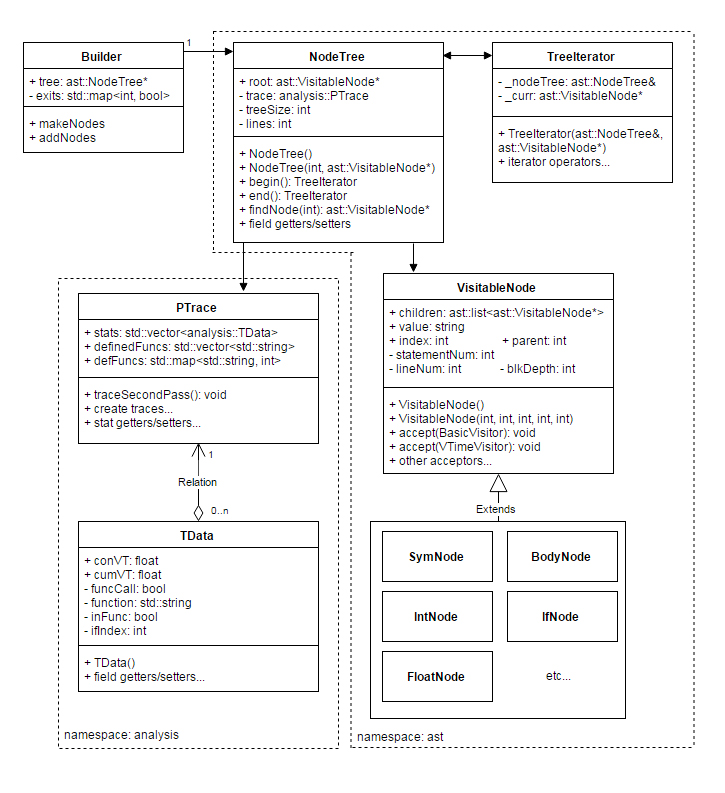
\includegraphics[width=0.9\textwidth]{images/timing.jpg}
	\caption{Tree UML} \label{tree}
\end{figure}
\newpage

\subsection{Timing Tree}
In calculating the virtual time at any point within the program the initial 
requirement is to parse the given program and store it for later access. A 
natural approach to this mimics compiler technology: we define some
grammar by which to parse our programs, and then build some Abstract Syntax Tree 
to store all of the program information. Once this 
is built successfully we are able to traverse the tree as often as we require 
to build the trace of the program. Figure \ref{tree} provides an overview of the 
different classes and their interactions for this section.

\subsubsection{Building the AST}
Whilst ruby has been valued in the Sonic-Pi project for its hugely forgiving
syntax in a classroom setting, this feature increases the difficulty of parsing 
it. The ability to write function calls either with or without parenthesis 
or ommit semi-colons between statements increases the complexity of the ruby 
grammar to the degree it was infeesable to write such a parser specifically 
for Sonic-Pi. However, given Sonic-Pi's ruby-like nature, we elected to use 
the open-source ruby-parser\footnote{As found at https://github.com/whitequark/parser}
for its simplicity and ease of set-up. It is relatively lightweight whilst 
still providing useful statistics such as line numbers, statement counts and
column numbers. In transferring this data to our own C++ application we are 
able to simplify the node count of our AST by wrapping certain nodes into 
tighter definitions. For example, the parser would output an integer as a node 
of type \texttt{int} with a child node holding the actual integer value. In 
building the AST of our C++ application we could wrap these definitions into 
a single node of type \texttt{IntNode} with held the integer value as a 
member field. \texttt{float} and \texttt{symbol} nodes acted in a similar
fashion:

% diagramtic example of a sym node
\begin{figure}[h!]
	\centering
	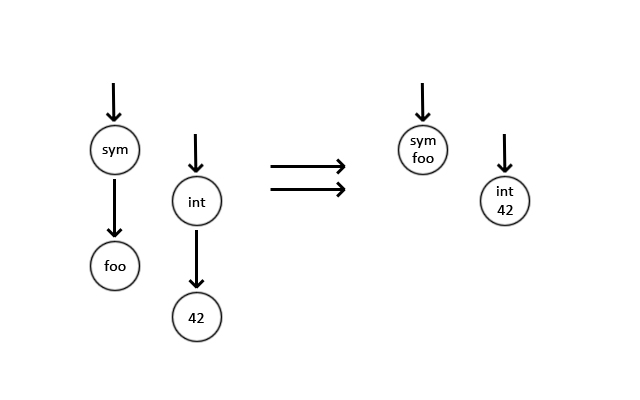
\includegraphics[width=0.85\textwidth]{images/SymInt.jpg}
	\caption{Node Wrapping} \label{symwrap}
\end{figure}

Statement lists are captured in the AST by nodes of type \texttt{begin} whilst
loops and function definitions are denoted by \texttt{block} types. 
\texttt{block} is a useful node type as it will always take three children, 
one describing the type of block, the second listing the arguments taken by 
the block and the final describing the root of the next statement list. 

% block node diagrams
\begin{figure}[h!]
	\centering
	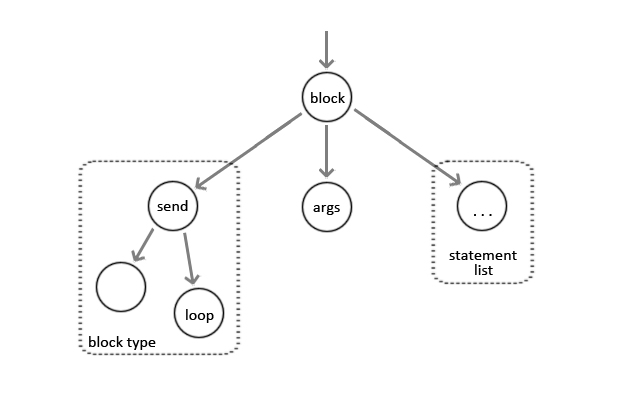
\includegraphics[width=\textwidth]{images/Block.jpg}
	\caption{Block Node Structure} \label{blocks}
\end{figure}

Whilst in the source code the end of a block is defined using the \texttt{end}
keyword, in the AST blocks can be viewed as self-contained trees; there is
no need for an \texttt{end}-type node. Most nodes are not necessarily aware
that they are in one block, with the parser providing no information
as to what scope level the code is at, at any given time. Entry to a block is
easy to detect, but leaving a block is more difficult. In general, when handling
whether a given node is within a particular function call we are required to
carry block index information and test whether parent indexes are different
at each node. It is not enough to store the block depth of each node in our AST
as sequential functions might think they are part of the same block; the
distinction is important later on when we start to calculate the contribution
of each function to the current virtual time of the program.

% block detection diagrams
\begin{figure}[h!]
	\centering
	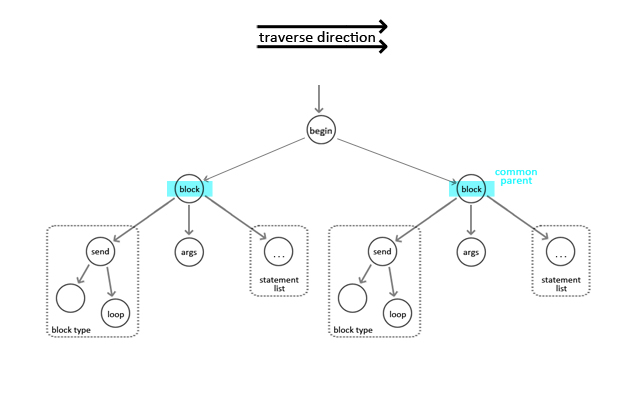
\includegraphics[width=\textwidth]{images/BlkDetection.jpg}
	\caption{Block Detection} \label{blockdetect}
\end{figure}



% some basic compiler type theory here would be good
% building of AST to traverse for information

\subsubsection{\texttt{pTrace}}
In describing the timing effects system we have implemented it is first necessary
to formalise the concept of the time system that Sonic Pi operates in. In providing
the abstract interpretation of a `time system' it becomes possible to prove the
`time safety' of the program by proving the semantics sound with respect to this 
system \cite{AOB14}. This enables developers to reason about their programs timing 
intuitively and allows us to reason about the safety of the program via static 
analysis.

The syntax of Sonic Pi V2.0 can be outlined simply.
\\
\begin{lstlisting}
	P ::= P; S | $\emptyset$
	S ::= E | $v$ = E
	E ::= sleep $\mathbb{R}_{{\geqslant}0}$ | A$^{i}$ | $v$
\end{lstlisting}

\texttt{P} represents a full program, 
\texttt{S} are statements (either self-contained expressions or pure bindings 
to variables), and \texttt{E} defines expressions. \texttt{A$^{i}$} is used to 
refer to all those operations that will not advance time, e.g. the 
\texttt{play} operation. In defining the syntax this way we are able to abstract 
over the operations that do not modify virtual time.

In distinguishing the real time elapsed by the program and the virtual time elapsed 
we write [\texttt{P}]$_{t}$ for the former and [\texttt{P}]$_{v}$ for the latter. 
Both of these abstract functions return time values and so are positive, 
real-number values.

\begin{blockquote}
	Virtual time is specified for Sonic Pi using the following cases:

	\begin{lstlisting}
     $\hphantom{..}$   [P; $v$ = E]$_{v}$ = [P]$_{v}$ + [E]$_{v}$
               [$\emptyset$]$_{v}$ = 0
         [sleep t]$_{v}$ = t
            $\hphantom{.....}$   [$v$]$_{v}$ = 0
            $\hphantom{...}$ [A$^{i}$]$_{v}$ = 0
	\end{lstlisting}
\end{blockquote}

% next go into how the trace is set up
% relate this breakdown of syntax into statements to how we store each statement
We action this specification by parsing our AST on a per-statement basis. Each 
\texttt{NodeTree} holds a reference to a \texttt{pTrace}, the data structure we 
use to store all of the important analysis results for the current program. The 
main fields of interest are a \texttt{std::vector} of \texttt{TData} pointers, a
\texttt{std::vector} of the names of functions defined and a \texttt{std::map} of 
function names to their virtual time contribution. Initially \texttt{pTrace} only
held a vector of integers, representing the contributing time, but this proved to 
be too little information on each statement. 

The program fills the information in \texttt{pTrace} based on the specification 
above. When the statement is a \texttt{sleep t} statement, it marks that the 
contributing virtual time, \texttt{conVT}, is of length \texttt{t}. Most other
statements are given a \texttt{conVT} of zero. To be able to report the total
virtual time of a run we also calculate the cumulative virtual time, \texttt{cumVT},
as we process the nodes. This is formalised by the sequence rule in our specification.

To start with a simple example, Snippet \ref{simpleLoop} shows the code for the
following simple trace.

\begin{multicols}{2}
	\begin{minipage}{0.4\textwidth}
		\begin{lstlisting}[style = sonicpi]

    loop do    # 1
      play 60  # 2
      sleep 2  # 3
      play 64  # 4
    end

		\end{lstlisting}
		\captionof{lstlisting}{Simple Loop} \label{simpleLoop}
	\end{minipage}

	\begin{minipage}{0.4\textwidth}
	\begin{lstlisting}
== Trace
[0] -                 
[1] conVT: 0, cumVT: 0, 
    isFunc: false, inFunc: false
[2] conVT: 0, cumVT: 0, 
    isFunc: false, inFunc: false
[3] conVT: 2, cumVT: 2, 
    isFunc: false, inFunc: false
[4] conVt: 0, cumVT: 2, 
    isFunc: false, inFunc: false
	\end{lstlisting}
	\end{minipage}

\end{multicols}

The information for each statement is mapped to the index of the same statement 
count. Index 0 is never filled as this is always assigned to the root node, due
to how we parse the tree information, and because it is natural for novice 
programmers to index from 1 rather than 0. Given this, we always skip handling
the first index of our trace because it is always a zero slot. Snippet 
\ref{simpleLoop} demonstrates quite neatly how simple it can be to collect the
cumulative virtual time as we iterate through the program, with it intially
seeming as simple as:
\\
\begin{lstlisting}
     [i].cumVT = [i].conVT + [i - 1].cumVT
\end{lstlisting}

\paragraph{Functions}
When we start to handle functions, this simple view of virtual time is not
quite robust enough. An example is given in Snippet \ref{doubleFunc} below.

It is entirely reasonable that someone might define multiple functions in this 
way when coding in a live arena. Even if it might be uncommon, it is a valid
program, making it important we can handle this type of situation. First we'll
provide the trace in full and then we will break down the approach and relevant 
theory.

\begin{minipage}{\textwidth}
	\begin{lstlisting}[style = sonicpi]
        define :first do       # 1
          play 60              # 2
        end
        
        first                  # 3
        second                 # 4
        play 60                # 5

        define :second do      # 6
          sleep 1              # 7
        end
	\end{lstlisting}
	\captionof{lstlisting}{Surrounding Functions} \label{doubleFunc}
\end{minipage}
\\
\begin{lstlisting}
    == Trace
    [0] -
    [1] conVT: 0, cumVT: 0, isFunc: false, inFunc: true
    [2] conVT: 0, cumVT: 0, isFunc: false, inFunc: true
    [3] conVT: 0, cumVT: 0, isFunc: true,  inFunc: false
    [4] conVT: 1, cumVT: 1, isFunc: true,  inFunc: false
    [5] conVT: 0, cumVT: 1, isFunc: false, inFunc: false
    [6] conVT: 0, cumVT: 0, isFunc: false, inFunc: true
    [7] conVT: 1, cumVT: 1, isFunc: false, inFunc: true
\end{lstlisting}

The issues that Snippet \ref{doubleFunc} identifies is how to insert the correct
amount of contributing virtual time into the trace when you might not have 
encountered the function being called. The simple way to handle this is by processing
the data in two passes. On the first pass of a program we collect information
such as which lines are function calls and what all of our function definitions
and times are. It is not printed in these traces but one of the extra things that
\texttt{TData} will hold is, if the current line is a function call, which function
does it call.

The trace after the first pass of this program looks as follows:
\\
\begin{lstlisting}
    == Trace
    [0] -
    [1] conVT:  0, cumVT:  0, isFunc: false, inFunc: true
    [2] conVT:  0, cumVT:  0, isFunc: false, inFunc: true
    [3] conVT: -1, cumVT: -1, isFunc: true,  inFunc: false
    [4] conVT: -1, cumVT: -1, isFunc: true,  inFunc: false
    [5] conVT:  0, cumVT: -2, isFunc: false, inFunc: false
    [6] conVT:  0, cumVT:  0, isFunc: false, inFunc: true
    [7] conVT:  1, cumVT:  1, isFunc: false, inFunc: true
\end{lstlisting}

Once this is processed it is again a simple case of adding up the cumulative virtual
time as we traverse the trace. \texttt{-1} is reserved as a keycode in tandem with
the \texttt{isFunc} marker; if a function has \texttt{conVT = -1} it means this
is a function call and will be processed in a later pass. It might seem like the 
keycode is useless in this case, but as the virtual time keycode is consumed during 
trace processing, it is useful to maintain the other boolean flag so that function 
calls are more easily identified afterwards.

The key idea is not to add together times from different blocks. The 
\texttt{inFunc} note helps with this, as we can detect when we are in a new block 
of the trace by what value that has. Notice that, in the above trace, index 6 
has a fresh \texttt{cumVT} value when compared with index 5.

\paragraph{Conditionals}
Similar to functions, we require a two pass approach to handle conditionals in the 
code. Take the following program code:

\begin{minipage}{\textwidth}
	\begin{lstlisting}[style = sonicpi]
        if true then      #1
            sleep 0.5     #2
        else
            sleep 1       #3
        end
	\end{lstlisting}
	\captionof{lstlisting}{Conditional} \label{conditional}
\end{minipage}

In practice it may be difficult to evaluate which branch of a conditional the
program is going to take. Instead the approach is to find the maximum virtual time 
of both branches and take the longest one. In terms of timing later in the program 
this could potentially throw developers on what the actual virtual time of the 
program will be if the \texttt{sleep} lengths differ by a sizeable margin. On the 
other hand this is a much safer model in terms of ensuring the time saftey of the 
program.

The trace for Snippet \ref{conditional} is:
\\
\begin{lstlisting}
    == First Pass Trace
    [0] -
    [1] conVT:  -2, cumVT: -2,   isFunc: false, inFunc: false
    [2] conVT: 0.5, cumVT: -1.5, isFunc: false, inFunc: false
    [3] conVT:   1, cumVT: -0.5, isFunc: false, inFunc: false

    == Second Pass Trace
    [0] -
    [1] conVT:  1, cumVT:    1, isFunc: false, inFunc: false
    [2] conVT: -3, cumVT: -1.5, isFunc: false, inFunc: false
    [3] conVT: -3, cumVT: -0.5, isFunc: false, inFunc: false
\end{lstlisting}

In the first pass of the trace, we mark the location of the if with the keycode 
-2. After this we calculate the virtual time of each branch and store the index 
for the last state of each branch in the \texttt{IfNode} at the root of this 
expression block. Similar to how block detection works, the end of an if-branch 
is detected when the next index in question has the same parent index, or one 
of greater value (or the program has finished in the case the conditonal is at 
the end of the program). With this, the second pass is simply a case of, on reaching 
a keycode of -2, set the result of whichever branch was longest.

\paragraph{Dead Code}

When calculating the virtual time of the program it is quite important not to 
take dead code into account. Dead code can easily push the trace into incorrect 
evaluation and make it difficult for the developer to calculate the time in their 
program. As well as this, being able to print when code will not be reached in a 
program is incredibly useful information for a developer to have in such an 
environment. Dead code can also be easy to locate thanks to the form of the program.

\begin{minipage}{\textwidth}
	\begin{lstlisting}[style = sonicpi]
      loop do
        play 60
        sleep 1
      end

      loop do
        play 60
        sleep 1
      end
	\end{lstlisting}
	\captionof*{lstlisting}{Dead Code} \label{dead}
\end{minipage}

We set \texttt{-3} to be the dead keycode and set all instances of \texttt{conVT} 
to this value when the statement is registered as dead. Here the second loop is 
obviously never going to be run, so we must remove this from consideration in our
trace. The trace makes a note of when it has seen a loop block and sets a boolean 
flag for dead code on hitting another loop block. Should the trace hit a 
\texttt{in\_thread} block or a \texttt{live\_loop} block then this flag is not set 
as these pieces of code can run in parallel.

\subsection{Session Graph}
Session Types describe communication protocols via message passing. In Sonic Pi
the message originates at a \texttt{cue} statement and is `consumed' by the
\texttt{sync} statement. Given this, we elect to transform the AST used in
timing analysis into a directed graph, consisting purely of \texttt{CueNode}s,
\texttt{SyncNodes}s and other \texttt{GraphNode}s to represent the passage
of time more generally in this analysis. Originally this third node type
was ommitted from the construction of the graph but on consideration of
message order in Sonic Pi it became clear that chronology was important 
information to maintain. This is discussed in more detail later in this section.

Presented next is the overall design of this section. Once the graph is
built the entry point to the analysis for this section calls on each sub 
graph to construct each session type and then the global type.

\begin{figure}[h!]
	\centering
	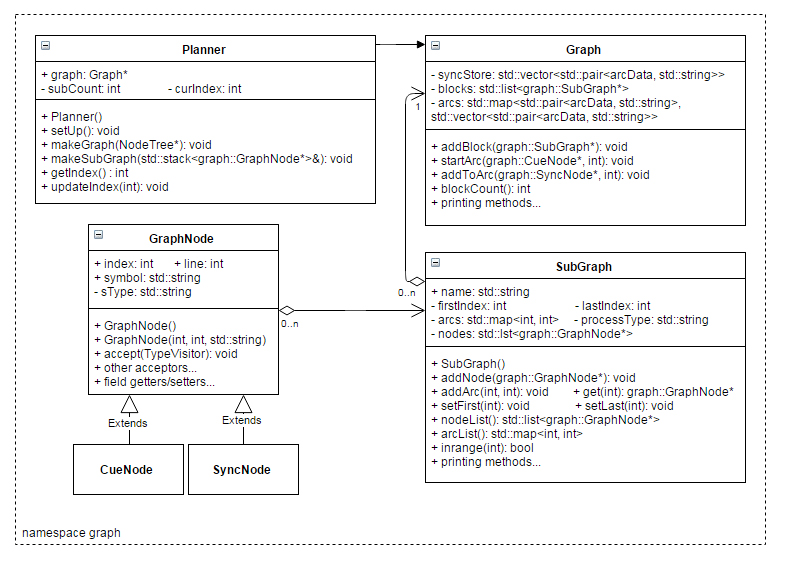
\includegraphics[width=\textwidth]{images/session.jpg}
	\caption{Graph UML} \label{graphUML}
\end{figure}

\begin{figure}[h!]
	\centering
	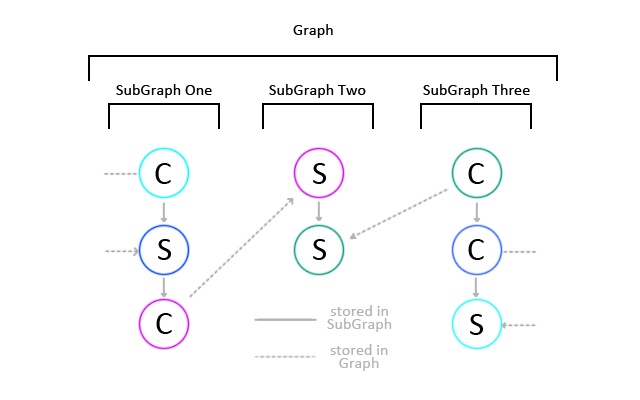
\includegraphics[width=\textwidth]{images/GSG.jpg}
	\caption{Graph Structure} \label{graphStructure}
\end{figure}

\subsubsection{Planning the Graph}
As shown by the Figure \ref{graphStructure}, each \texttt{Graph} is constructed as
a list of \texttt{SubGraph}s where each \texttt{SubGraph} represents
one process within the program. The idea behind this is to maintain
the chronology of the nodes in each process and to enable easy analysis
of the program on a per-process level. \texttt{SubGraph} handles the construction
of local types while the \texttt{Graph} class handles the global type.

\paragraph{Initial Design}
In defining the session types we can consider a modified version of the syntax 
of Sonic Pi V2.0 defined earlier.
\\
\begin{lstlisting}
	P ::= P; S | $\emptyset$
	S ::= E  | $v$ = E
	E ::= sleep $\mathbb{R}_{{\geqslant}0}$ | cue $v$ | sync $v$ 
	    | A$^{i}$ | $v$
\end{lstlisting}

We expand the syntax to define \texttt{cue} and \texttt{sync} which operate on
some variable name, $v$. We maintain our definition of \texttt{sleep} in this syntax 
as it is a useful tool in our reasoning. \texttt{A$_{i}$} is thus the set of all 
operations that either do not advance time or do not consist of some communication
primitive. In this way we can abstract over the operations that do not contribute 
to communications.

\begin{minipage}{\textwidth}
	\begin{lstlisting}[style = sonicpi]
           # P0                        # P1
           in_thread do                in_thread do 
             loop do                     loop do
               cue :B                      cue :A 
               sync :A                     sleep 1
               sleep 1                     sync :B
               play 63                     sleep 0.5
             end                         end
           end                         end
	\end{lstlisting}
	\captionof{lstlisting}{Forming Types} \label{formTypes}
\end{minipage}

For the following section, the base set of syntax we use to describe our session
types are as follows\footnote{Other sets used are \emph{constants}, 
\emph{expressions}, and \emph{process variables} but we do not need to consider 
these for the language constructs discussed in this report.}:

\begin{itemize}[noitemsep]
  \item[] \emph{names}: ranged over by \emph{a,b...}
  \item[] \emph{channels}: ranged over by \emph{k, k'...}
  \item[] \emph{variables}: ranged over by \emph{x, y...}
  \item[] \emph{labels}: ranged over by \emph{l,l'...}
\end{itemize}

The final set of interest is that of \emph{Processes}, ranged over 
by \texttt{P, Q...}. For this discussion we define the following aspects 
of the \emph{Process} grammar:
\\
\begin{lstlisting}
    P ::= k![$\tilde{e}$]. P                    data sending
        | k?($\tilde{x}$) in P                  data reception
        | def D in P                 recursion
\end{lstlisting}
\begin{lstlisting}
    D ::= X$_1$($\tilde{x}_1\tilde{k}_1$) = P1 and ...           declaration for recursion
                and X$_n$($\tilde{x}_n\tilde{k}_n$) = P$_n$ 
\end{lstlisting}

``$|$'' is the weakest association; the others listed have the same association. 
Parenthesis denote binders which bind the corresponding free occurrences. We use 
standard simulataneous substitution, written $ $. The sets of free 
names/channels/variables of, for example program \texttt{P}, are written as 
\texttt{fn(P)}, \texttt{fc(P)}, and \texttt{fv(P)} respectively. Processes without 
free variables or free channels are called programs.

This project uses the multi-party session typing paradigm, which presents a slight
improvement to this syntax, allowing our communication to occur between more
than two \emph{participants}. \emph{Participants} are the set ranged over by 
\emph{p, q,...}
\\
\begin{lstlisting}
    P ::= c!<p,e>.P             value sending
        | c?(p,x).P             value reception
\end{lstlisting}

With this we can now state which of our participants we are sending our message
to and on which channel. With this we are now able to begin typing our programs.

When forming the types of threads, the program of Snippet \ref{formTypes}
would produce types of the form:
\\
\begin{lstlisting}
    P0 :=  B:(P0P1)!.A:(P1P0)?
    P1 :=  A:(P1P0)!.B:(P0P1)?
\end{lstlisting}

`.' is defined as composition, enabling us to string together our types as
a simple sequence.

This is the manner in which the library chooses to define the types as this
results in a simpler string to parse. In these types, \texttt{A} and \texttt{B} 
are acting as the names of the channel being used to send and receive data.
The first \texttt{P} instance enclosed in each parenthesis is the sender, the 
second is the receiver. In printing the types in this manner we are able to 
store each type in the \texttt{SubGraph} it belongs to and comparison of types
can be decided quickly with index access to the first and last chars, rather than
another position in the string.

To begin illustrating global types by example, we present the standard 
two-buyers-protocol.

First \texttt{B1} sends a title to \texttt{S} and in responce \texttt{S}
sends a quote to both \texttt{B1} and \texttt{B2}. \texttt{B1} will then
suggests what contribution it can make to \texttt{B2} who will either
accept this amount and coordinate the purchase with \texttt{S}, or it will
abort the discussion. Decomposing this into three binary session types
could be logically very difficult, and most likely we would lose some of
the essential sequencing information in the process. Instead, let us transform
this scenario into the following global type. Global types are presented as
numbers, so a clear key is also provided:
\\
\begin{lstlisting}
    1)  1 $\rightarrow$ 3 : $\langle$string$\rangle$                         B1 = 1
    2)  3 $\rightarrow$ 1 : $\langle$int$\rangle$                            B2 = 2
    3)  3 $\rightarrow$ 2 : $\langle$int$\rangle$                             S = 3
    4)  1 $\rightarrow$ 2 : $\langle$int$\rangle$
    5)  2 $\rightarrow$ 3 : { ok: 2 $\rightarrow$ 3 : $\langle$string$\rangle$. 3 $\rightarrow$ 2 : $\langle$date$\rangle$. end,
                quit: end }
\end{lstlisting}

In our analysis, a message can defined a passing from process \texttt{P0}
to process \texttt{P1}, written \texttt{P0->P1}, if the types in processes 
\texttt{P0} and \texttt{P1} dual each other. The algorithm we have for processing
each type starts in the first type of each block and stores each token. If
the next token is a dual of any of the tokens in our store we write out the
next part of the global type and remove them from the store. If not, we
remove any \texttt{cue} types from the current store, keep the \texttt{sync} 
types and then place the current token at the top of the store and continue 
until all type block have been consumed.

% diagram of internal graphs here, showing that nodes in these graphs 
% are chronological
\begin{figure}[h!]
	\centering
	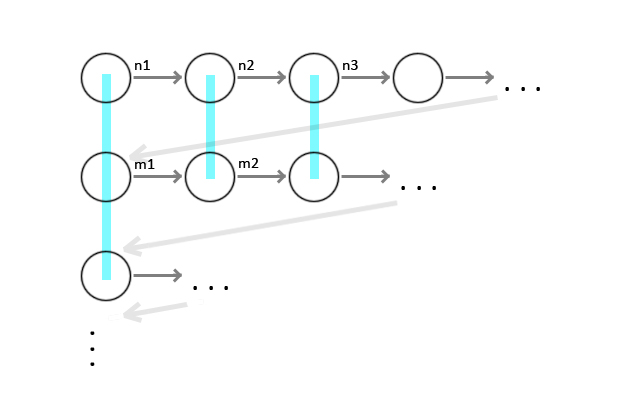
\includegraphics[width=\textwidth]{images/GraphOneFix.jpg}
	\caption{Node Chronology} \label{nodegraphone}
\end{figure}

The reason we may process tokens in this way is demonstrated in Figure 
\ref{nodegraphone}. A Sonic Pi program will always increment its virtual 
time as we run through a program. \texttt{SubGraph}s are written in the order 
they are defined in the source by line number. Given this, within a 
\texttt{SubGraph} if \texttt{n1.index < n2.index}, \texttt{n1} has resolved 
first. In later sections we will refer to this as the `horizontal' relationship 
between nodes. In two concurrent \texttt{SubGraph}s, \texttt{n.index < m.index} 
and \texttt{n} will be resolved first by the interpreter but they may have the 
same virtual time within the program, thus they are compared to each other as 
well as those tokens processed one previously. We will refer to this as the 
`vertical' relationship between nodes and is demonstrated in Figure 
\ref{nodegraphone} by the blue bar linking the different groups together.

There is a small limitation in this design as it will allow certain untypable
programs to be typed.

An example of this can be shown with the deadlocking code from previously,
shown again in Snippet \ref{typelock}. As it is, this will produce the same session
graph as Snippet \ref{formTypes}, which produces a feesable global type.
The actual result for this should be untypable as both loops will become stuck
at each \texttt{sync} node. 

\begin{minipage}{\textwidth}
	\begin{lstlisting}[style = sonicpi]
	live_loop :foo do
	    play :e4, release: 0.5
	    sleep 0.5
	    sync :bar
	end

	live_loop :bar do
	    sample :bd_haus
	    sleep 1
	    sync :foo
	end
	\end{lstlisting}
	\captionof{lstlisting}{Deadlock - Types Under This Approach} \label{typelock}
\end{minipage}

\paragraph{Keeping Time}
To combat this we updated the construction of the graph to take into account
a very basic notion of the passage of time. As the AST is being traversed, each
instance of a \texttt{BodyNode} of value \emph{sleep} will create an empty
\texttt{GraphNode} in the session graph. This does not break the order relation
described previously but it does change the grouping of the `vertical' 
relationship of the nodes. Rather than mapping each column as one relation, with
the total set of relationship being equal to the maximum number of types in
any one \texttt{SubGraph}, each `vertical' relation can be defined as the
set of nodes between each \emph{time} node.

% updated graph diagram here
% highlights each vertical relation group
\begin{figure}[h!]
	\centering
	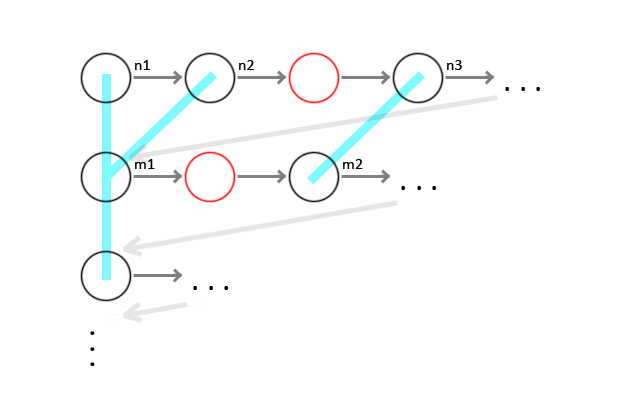
\includegraphics[width=\textwidth]{images/GraphTwo.jpg}
	\caption{Fixed Node Chronology}
\end{figure}

Refering back to Snippet \ref{formTypes}, the program graph constructed now takes
the form:
\\
\begin{lstlisting}
  P0 :=  B:(P0P1)!.A:(P1P0)?.time
  P1 :=  A:(P1P0)!.time.B:(P0P1)?.time
\end{lstlisting}

More importantly the program from snippet 12 will look as follows:
\\
\begin{lstlisting}
  foo := foo:(P0P1)!.time.bar:(P1P0)?
  bar := bar:(P1P0)!.time.foo:(P0P1)?
\end{lstlisting}

As before we process each block one `vertical' relation at a time. We take
care in this iteration to make a note when a block is stuck at a \texttt{sync}
node as we should not process any further tokens from this block. Rather than
processing until the each of each token block, we process the first token group
again in the event any trailing syncs would be triggered by the next loop. In
the event we run into the same \texttt{sync} node that we are currently blocked
on then we are able to return that this global type is not typeable.

% new graph style

\subsubsection{Global Construction}


% recap important parts of MPST
% start by explaining the theory of the approach

% what information was important, why did this link up with session graph?

As discussed previously in Section 4.2.1, the usual approach to multi-party session 
types is to construct the global type of your program and then project the 
individual process types from that. With this one can then write each process, 
ensuring that all communication protocols remain consistent as development 
proceeds. Projection is a simple and decidable approach to session times.

The global types describe the various actions of a participant \texttt{p} sending
either a value of a given Sort, a channel of a given Type, or some label to the
partcipant \texttt{q} and then interaction continues according to the following
global type \texttt{G}. The grammar we are interested in here is as follows:
\\
\begin{lstlisting}
    G ::= p $\rightarrow$ q : $\langle$S$\rangle$.G
        | p $\rightarrow$ q : $\langle$T$\rangle$.G
        | $\texttt{\textbf{t}}$
        | end
\end{lstlisting}

To understand how we build a global type from decomposed local types, we first 
present the simpler operation of \emph{projection}. The global type is the
description of the program as the whole. It shows which participants 
communication with which and what data they pass between each other. The decomposed
local type describes the interaction that specific process is aware of. The 
definition of \emph{projection} follows:

\begin{blockquote}
  \textbf{Definition 1:} \emph{The projection of a global type \texttt{G} onto 
  a particiapnt \texttt{q} is defined by induction on \texttt{G}}:
\end{blockquote}
\begin{align*}
  (\texttt{p} \rightarrow \texttt{p'}:\texttt{<U>}.\texttt{$G$'}) \upharpoonright \texttt{q = }  
  \begin{cases}
\hspace{5pt} !\langle \texttt{p',U} \rangle (\texttt{$G$'}\upharpoonright \texttt{q}) \hspace{22pt}if \hspace{5pt} \texttt{q = p} \\
\hspace{5pt} ?(\texttt{p',U}) (\texttt{$G$'}\upharpoonright \texttt{q}) \hspace{20pt}if \hspace{5pt} \texttt{q = p'} \\
\hspace{5pt} \texttt{$G'$}\upharpoonright \texttt{q} \hspace{65pt} otherwise
  \end{cases}
\end{align*}
\begin{align*}
  \texttt{t} \upharpoonright \texttt{q = t} 
  \hspace{40pt} \texttt{end} \upharpoonright \texttt{q = end}
\end{align*}

This approach is not so feesable in this instance as we have already been 
presented with the full source. Instead we are required to build the global
type from the individual process types provided, the aim being to verify
the communication of the program through this process. This consists largely of 
matching operations on the channels they operate on. Whilst notably more
difficult, this approach is also, thankfully, proveably decidable. There is
no situation where any algorithmic approach to the problem will not terminate
with some answer. In the cases where our program's global type is not
typable, this suggests some communication error within the provided program.

Given the dual types \texttt{A:P0P1?} and \texttt{A:P0P1!} we can transform 
this into the global typing \texttt{P0->P1}, representing the fact that a 
messagevis being transfered from \texttt{P0} to \texttt{P1}. \texttt{A} is not
represented within this global type as it acts as the name of the channel on
which the message is being sent. In this sense you can consider Sonic Pi
to be a series of zero size messages being sent on each channel between
each process.

Interestingly the syntax of Sonic Pi allows for some interesting situations,
some of which are not technically typable in strict Session Types but are
perfectly valid, and sometimes useful, situations to occur in Sonic Pi.

The first such situation we consider is when we have several \texttt{cue}
signals with the potential to trigger one \texttt{sync}.



In this scenario the \texttt{sync} in \texttt{P1} may be triggered by either
of the \texttt{cue}s present in the other two threads. Whilst unusual,
it is not unreasonable to suggest this is a valid program. It may be that the
developer has set up the rest of the program code so that threads \texttt{P1} 
and \texttt{P2} alternate for each loop that \texttt{P1} performs. The use
of this in a musical sense could be an interesting drum riff to underpin the
song, or some decorative melodies. To capture this information Sonic Pi 
proposes an `\emph{or}' type, denoted by \texttt{||}. 


\begin{minipage}{\textwidth}
	\begin{lstlisting}[style = sonicpi]
    # P0                # P1                # P2
    in_thread do        in_thread do        in_thread do
      loop do             loop do             loop do
        cue :A              sync :A             cue :A
        sleep 1             sleep 1             sleep 1
      end                 end                 end
    end                 end                 end
	\end{lstlisting}
	\captionof{lstlisting}{One \texttt{sync}, multiple \texttt{cue}}
\end{minipage}


Given this notation the
decomposed types for this set of threads is:
\\
\begin{lstlisting}
  P0 := A:(P0P1)!
  P1 := A:(P0P1||P2P1)?
  P2 := A:(P2P1)!
\end{lstlisting}

Notice in this instance we are referring only to the `strict' types of each 
process, rather than our graphical representation of the process, so the
\texttt{time} elements discussed in the previous section have been ommitted 
for this discussion.



In terms of processing the global type, when each of these types line up
into the same `vertical' relationship, the type constructed has the form 
\texttt{(P0||P2)->P1}. The algorithm discussed previously does not need
adapting to handle this new type form. The tokens are not removed from the
stored pool until every node in the group has been processed. We are only
required to add in some new code to handle the case where we have detected
the extra information else we may actually print the types as a composition,
\texttt{P0->P1.P2->P1}. This is a valid session type but is not an accurate
definition for this situation.

The other situation we considered is when one \texttt{cue} can trigger
multiple \texttt{sync} statements. This is equally as untypable in strict
session types but equally as viable from a musical point of view. The developer
may have multiple melodies playing concurrently that should all sync onto the
same drum beat.

\begin{minipage}{\textwidth}
	\begin{lstlisting}[style = sonicpi]
    # P0                # P1                # P2
    in_thread do        in_thread do        in_thread do
      loop do             loop do             loop do
        sync :A             cue :A              sync :A
        sleep 1             sleep 1             sleep 1
      end                 end                 end
    end                 end                 end
	\end{lstlisting}
	\captionof{lstlisting}{One \texttt{cue}, multiple \texttt{sync}}
\end{minipage}

In this situation we propose a simple `\emph{and}' type. \texttt{cue} is an
asynchronous message that propogates out to all processes currently waiting.
Given this, the \texttt{cue} present in \texttt{P1} will trigger the \texttt{sync}
in \texttt{P0} \emph{and} the \texttt{sync} in \texttt{P2}. The types we 
print for this are as follows:
\\
\begin{lstlisting}
  P0 := A:(P1P0)?
  P1 := A:(P1P0&&P1P2)!
  P2 := A:(P1P2)?
\end{lstlisting}

As before, the algorithm for creating global types from this type set is not
affected. The \texttt{sync} statements will either be in the store from a previous
iteration of the algorithm or be handled as all statements from the same `vertical'
relationship will be processed. The global type for this situation will be printed
as \texttt{P1->(P0\&\&P2)}. In the event these statements are separated by time
progression, the type will print as the usual global type involving two processes.
\texttt{sync} statements will still be stored as described earlier, either to be
consumed by a later \texttt{cue} of the correct dual typing or to be hit again
and processed as an untypable program.

On initial consideration one might define the \texttt{||}-type as a dual of the
\texttt{\&\&}-type, and vis versa, but this is inaccurate for the context in which
they are used. The main component of these types is still the act of sending or
receiving a message, so dual typings are still based off of the dual relationship
of `\texttt{?}' and `\texttt{!}'. The two types we introduce here are more like
a `typing sugar' to describe situations where a process can send and received
multiple messages at the same time. This is not a situation that session types
usually handle. Session Types are defined by their use of message queues, sending
message packets (be they single packets or multiple) in sequence along the 
\emph{same} channel to \emph{single} receivers. It does not define a situation
where one can trasmit a message on one channel to multiple places. In this case
this projects presents an interesting evolution of session types for this field.
We have implemented multiple modes that our project can operate under to reflect
this, so developers can choose to analysis under `strict' typing or under the
`Sonic Pi' typing outlined here.
\newpage

\paragraph{Sub-Typing}
\begin{multicols}{2}
Introducing the concept of time progression into the graph also handles one other
case that the initial column approach did not.

Under the initial algorithm, both \texttt{cue} statements in snippet 16 would be
processed and then discarded, as \texttt{cue} statements do not persist in the 
statement store. However, these statements all execute at the same virtual time 
in the program; both \texttt{cue}s will trigger both \texttt{sync}s in the Sonic 
Pi environment. 
\\
\begin{lstlisting}
  P0 := B:(P0P1)!.A:(P1P0)?
  P1 := A:(P0P1)!.B:(P0P1)?
\end{lstlisting}

In `strict' session types this is inaccurate:

$\hphantom{tabs}$ \texttt{B:(P0P1)!.A:(P1P0)?} 
\\ $\hphantom{tabular} \neq$ \texttt{dual(A:(P0P1)!.B:(P0P1)?)}

The accurate type for the second process would be \texttt{B:(P0P1)?.A:(P0P1)!}, 
(or one could keep \texttt{P1} unchanged and swap the terms in the other process). 
To handle this, the project makes use of sub-typing the \texttt{cue} type.

	\begin{minipage}{0.5\textwidth}

		\begin{minipage}{\textwidth}
			\begin{lstlisting}[style = sonicpi]
	# P0 
	in_thread do
	  loop do   
	    cue :B  
	    sync :A 
	    play 60 
	    sleep 0.5 
	  end 
	end           


	# P1
	in_thread do
	  loop do
	    cue :A
	    sync :B
	    play 64
	    sleep 0.5
	  end
	end
			\end{lstlisting}
			\captionof{lstlisting}{Sub-Typing \texttt{cue}}
		\end{minipage}

	\end{minipage}
\end{multicols}

The formal outline for this feature is:
\\
\begin{lstlisting}
     A!.P <: P.A!
\end{lstlisting}

Given this we may say that:
\\
\begin{lstlisting}
     A:(P0P1)!.B:(P0P1)? <: B:(P0P1)?.A:(P0P1)!
     B:(P0P1)!.A:(P1P0)? = dual(B:(P0P1)?.A:(P0P1)!)

    $\therefore$ B:(P0P1)!.A:(P1P0)? $\cong$ dual(A:(P0P1)!.B:(P0P1)?)
\end{lstlisting}

Sub-typing is a useful relation to define within session types, see 
\cite{HYC08, MY15, MYH09}, and is based on the notion that correctness will 
always be maintained so long as input order is not disrupted in the message 
queue. Here, our subtype is based on operations occuring at the same `virtual 
time', so we may consider operation ordering to be maintained in this instance. 

\subsection{Integration}

The Sonic Pi IDE has two core sections: Server and GUI. The server is written on 
top of the SuperCollider synthesizer and implemented in Ruby whilst the GUI is 
built on the Qt framework and thus written in C++.

Integrating this library comes in two stages. Firstly delving into the server to 
locate the area where the code is evaluated before being made into music. Sonic 
Pi's code evaluation is handled by a \texttt{spider} module, which holds the main 
evaluation method. This module also has the capacity to print straight into the 
IDE's output log widget, making the first step of relaying information to the 
screen very simple. The pseudo code for this \texttt{spider} integretion is very
simple.
\\
\begin{lstlisting}[style = sonicpi]
    def __spider_eval(code)
        # thread setup
        # ...
        code = Preparse(code)
        analysis_output = __verify_code(code)
        __info(analysis_output)
        # ...
        # message handling and thread handling
        # ...
    end
\end{lstlisting}

Secondly, to better display the timing effects information, we choose to define 
a new output widget in the \texttt{mainWindow} class of the gui. Qt thankfully 
simplifies the GUI process considerably, meaning it is not too difficult to produce
an attractive addition in keeping with the existing theme of Sonic Pi. We are 
also able to mimic the \texttt{\_\_info} method we use to print to the output log
to be able to print our timing information into our new widget.

% basic outline of sonic pi
% The basic architecture of Sonic Pi can be broken into the server side of the application and the gui. The gui brings a hard dependency on the Qt framework, implemented in C++, whilst the server application is developed with ruby. 
% In order to generate and manipulate sounds, Sonic Pi is implemented in terms f the SuperCollider synthesis server which provides the ability to define arbitiary synthesiers and trigger and manipulate them in real time\cite{AB13}
% The main entry point for Sonic Pi lies in the spider_eval method of the spider class
% defined in the server modules. It is here we intercept the currently played pieces of music and run our own analysis modules.

% once the hookup is done write out the code examples of how messages are passed along
% maybe make a basic diagram of Sonic Pi interactions with/without our project

\newpage

\section{Evaluation}
\thispagestyle{empty}
\subsection{Ruby/C++11 \& Performance}
In evaluating our project it is necessary to question whether the tools used were
in fact the right ones for the given task. We have implemented an analysis library
in C++11 which successfully hooks into the existing Ruby modules. This library
could easily have been written in Ruby, saving the need for the extra steps
of converting the data from one type to another. 

The reason for our
use of C++11 is to take advantage of the speed of the language. The tool used for
for the data transfer here is Ruby Rice, a type-safe and exception-safe interface
between C++ and Ruby's C API\footnote{As found at https://github.com/jasonroelofs/rice}.
Other similar tools for this are Ruby Inline and Ruby's FFI tool. Below is a table
of their relative performances based on some short implementations of fibonacci, 
factorial and pow methods.

\begin{table}[h]
	\centering
	\caption{Ruby Interfacing Performances \cite{amber}} \label{ruby}

	\begin{tabular}{llll}
	          \\
	          & Ruby Inline & Ruby Rice   & Ruby FFI  \\ \hline
	          \\
	factorial & 0.026175138 & 0.197720523 & 0.014882004  \\
	fibonacci & 0.026792521 & 0.202714029 & 0.018928646  \\
	pow       & 0.03252452  & 0.211258897 & 0.023082315
	\end{tabular}
\end{table}

Disappointingly, Ruby Rice performs the slowest of this tools in this scenario. 
On standard desktop environments this amount is little cause for concern as both
the Sonic Pi IDE and the extention library run smoothly with no trouble. The average
processing time for this project on [desktop specs] is [time here]. This being said,
it is important to remember that these results are based on very simple mathematical 
methods, not something you would likely use embedded C for in a real project.

The crucial question is how well this runs on an actually Raspberry Pi as this is
the target device for the language. When run on a recent Raspberry Pi 2, average
performance is [time here].

While these results are strong it doesn't go the full distance in answering if the
library was better served implemented in Ruby or C++11. The library as it is, is able
to take advantage of many useful features of C++11; notably the host of available
data structures for each task. That said, whilst Ruby only has Array and Hash 
structures avaiable to it, Ruby does still have the concept of classes and modules 
meaning our current class setup is largely portable to a Ruby environment. 
Unfortunately there has not been time thus far to test how fast a Ruby implementation
is compared to the current project state.

Another reason for the use of C++ was the hopes to make greater use of the boost
graph library\footnote{http://www.boost.org/doc/libs/1\_58\_0/libs/graph/doc/}. 
In implementing the graph analysis with this it would have been useful to have
immediate access to such things as the iterators and many different graph algorithms
(djisktra, etc...) that bgl implements. Currently the \texttt{SubGraph} structure
we have does not translate well into bgl. It is possible to compile this 
implementation but data is tricky to initialise and access later on. In the interest
of time this idea was shelved and a much simpler graph structure was put in place.
Despite the large code dependancy bgl can introduce, it may be interesting to
revisit the idea in the future, should the search-algorithms it has ready-implemented
become required.

% comments on the three different methods available?

% notes on speed of data transfer between ruby and C application

% mention other ruby parser options -> maybe find some benchmark stats

% -> attempt at boost library and why that was dropped?


\subsection{Correctness}
To confirm the correctness of our approach we have built a systematic testing
environment. It is important when building verification tools to have a series
of programs to test results with and ensure any interesting edge cases of behaviour
can be detected and dealt with. In this system we been with a series of simple
programs, testing simple chords and sequencing, single function detection, etc...,
before moving into more complex programs. At the later end of the suite we test
on a full musical piece, taken from the samples provided in the Sonic Pi IDE. In
presenting these results, we provide the source for the program, an expected trace
result and then our actual analysis result.

All codes written here can be repeated with notes in MIDI format (\texttt{:C4}, 
for example) and will produce the same results as the integer format presented.
The reason for this is that the note values are wrapped into \texttt{SymNode} types 
in the same way the numbers are wrapped into the \texttt{IntNode} type. This means 
the analysis approach for them is the same and the results are deterministic.
Session analysis results are only presented when relevant to the code being
discussed, as the library is quite efficient at setting empty types. Where functions
are not being tested, trace information such as whether the statement is a function 
call or not is ommitted for brevity.

\subsubsection{Chords}

\begin{minipage}{\textwidth}
	\begin{lstlisting}[style = sonicpi]
      play 60
      play 62
      play 64
	\end{lstlisting}
	\captionof*{lstlisting}{Chord Test Code}
\end{minipage}
\\
\begin{lstlisting}
    == Expected Trace               == Actual Trace
    [0] -                           [0] -
    [1] conVT: 0, cumVT: 0          [1] conVT: 0, cumVT: 0
    [2] conVT: 0, cumVT: 0          [2] conVT: 0, cumVT: 0
    [3] conVT: 0, cumVT: 0          [3] conVT: 0, cumVT: 0
\end{lstlisting}

This trace correctly confirms that the given program does not advance virtual time 
at any points, reporting a statement length of three.

\subsubsection{Sequences}
\begin{minipage}{\textwidth}
	\begin{lstlisting}[style = sonicpi]
      play 60
      sleep 1
      play 62
      sleep 1
      play 64
	\end{lstlisting}
	\captionof*{lstlisting}{Sequence Test Code}
\end{minipage}
\\
\begin{lstlisting}
    == Expected Trace               == Actual Trace
    [0] -                           [0] -
    [1] conVT: 0, cumVT: 0          [1] conVT: 0, cumVT: 0
    [2] conVT: 1, cumVT: 1          [2] conVT: 1, cumVT: 1
    [3] conVT: 0, cumVT: 1          [3] conVT: 0, cumVT: 1
    [4] conVT: 1, cumVT: 2          [4] conVT: 1, cumVT: 2
    [5] conVT: 0, cumVT: 2          [5] conVT: 0, cumVT: 2
\end{lstlisting}

Here we correctly identify five statements, two of which advance time. The final 
length of virtual time is the sum of all \texttt{sleep} statements used. Here this 
is accurate as it is a simple sequence of operations.

\subsubsection{Loops}
\begin{minipage}{\textwidth}
	\begin{lstlisting}[style = sonicpi]
      loop do
        play 60
        sleep 1
      end
	\end{lstlisting}
	\captionof*{lstlisting}{Loop Test Code}
\end{minipage}
\\
\begin{lstlisting}
    == Expected Trace               == Actual Trace
    [0] -                           [0] -
    [1] conVT: 0, cumVT: 0          [1] conVT: 0, cumVT: 0
    [2] conVT: 0, cumVT: 0          [2] conVT: 0, cumVT: 0
    [3] conVT: 1, cumVT: 1          [3] conVT: 1, cumVT: 1
\end{lstlisting}

The trace identifies three statements, where on is the commencement of the loop. 
By the end of the loop, virtual time will have advanced by one, as printed by 
our analysis.

\begin{minipage}{\textwidth}
	\begin{lstlisting}[style = sonicpi]
      loop do
        play 60
        sleep 1
        loop do
          play 64
          sleep 1
        end
      end
	\end{lstlisting}
	\captionof*{lstlisting}{Nested Loop Test Code}
\end{minipage}
\\
\begin{lstlisting}
    == Expected Trace               == Actual Trace
    [0] -                           [0] -
    [1] conVT:  0, cumVT: 0         [1] conVT:  0, cumVT: 0
    [2] conVT:  0, cumVT: 0         [2] conVT:  0, cumVT: 0
    [3] conVT:  1, cumVT: 1         [3] conVT:  1, cumVT: 1
    [4] conVT:  0, cumVT: 1         [4] conVT:  0, cumVT: 0
    [5] conVT:  0, cumVT: 1         [5] conVT:  0, cumVT: 0
    [6] conVT:  1, cumVT: 2         [6] conVT:  1, cumVT: 1
\end{lstlisting}

This has highlighted a limitation in the current iteration. The contributing time 
detection works but the cumulation does not accurately detect nested blocks. 
Instead it sees each new block and starts the cumulation fresh, as those they were
sequential blocks. This shows the project is not currently making the most use out 
of the block level data that is taken during the construction of the AST. This could 
be fixed by testing whether a new block has a higher level than the previous token.
In the event it does the trace can skip starting a fresh \texttt{cumVT} value, if it 
is equal or less than then the old behaviour applies. 

\begin{minipage}{\textwidth}
	\begin{lstlisting}[style = sonicpi]
      5.times do
        play 60
        sleep 1
      end
	\end{lstlisting}
	\captionof*{lstlisting}{`Timed' Loop Test Code}
\end{minipage}
\\
\begin{lstlisting}
    == Expected Trace               == Actual Trace
    [0] -                           [0] -
    [1] conVT: 5n, cumVT: 0         [1] conVT: -1, cumVT: -1
    [2] conVT:  0, cumVT: 0         [2] conVT:  0, cumVT: -1
    [3] conVT:  1, cumVT: 1         [3] conVT:  1, cumVT:  0
\end{lstlisting}

This loop structure is currently not handled correctly. Ideally, since this is set 
to run a set number of times, once the trace has processed the loop length, there 
should be some stored multiplier that can be used to accurately set the 
\texttt{cumVT} value after the loop to a much higher number (in this test case, the 
next \texttt{cumVT} would be \texttt{5} plus whatever the next \texttt{conVT} 
evaluates to).

What actually happens is \texttt{times} is registered as a function. In ruby terms,
this is technically a function being sent the value 5 to act on. What we may do in 
future is set another keycode (-4) which tells the second pass of the trace that 
there is an argument to this loop that it must multiply the total loop time by and
then use this value in subsequent trace calculations.

\begin{minipage}{\textwidth}
	\begin{lstlisting}[style = sonicpi]
      5.times do
        play 60
        sleep 1
        5.times do
          play 64
          sleep 1
        end
      end
	\end{lstlisting}
	\captionof*{lstlisting}{Nested `Timed' Loop Test Code}
\end{minipage}
\\
\begin{lstlisting}
    == Expected Trace               == Actual Trace
    [0] -                           [0] -
    [1] conVT: 5n, cumVT: 0         [1] conVT: -1, cumVT: -1
    [2] conVT:  0, cumVT: 0         [2] conVT:  0, cumVT: -1
    [3] conVT:  1, cumVT: 1         [3] conVT:  1, cumVT:  0
    [4] conVT: 5n, cumVT: 1         [4] conVT: -1, cumVT: -1
    [5] conVT:  0, cumVT: 1         [5] conVT:  0, cumVT: -1
    [6] conVT:  1, cumVT: 2         [6] conVT:  1, cumVT:  0
\end{lstlisting}

This trace carries forward the limitations of both nested and timed traces shown 
previously.

There is also the ability to make a parameterized loop with \texttt{n.times},
where \texttt{n} has been passed to the function the loop is contained in. This
test is not included here for brevity, as the results are similar those presented
here. The reason for this is whilst the library can see the symbols easily,
the code is currently not processing it. For this reason, parameterized code
is processed as if they were unparameterized. In the case of loops, this means
all loops are handled once and VT is printed as though each loop only occured once.

\subsubsection{Threads}
\begin{minipage}{\textwidth}
	\begin{lstlisting}[style = sonicpi]
      in_thread :foo do
        play 60
        sleep 1
      end
	\end{lstlisting}
	\captionof*{lstlisting}{Thread Test Code}
\end{minipage}
\\
\begin{lstlisting}
    == Expected Trace               == Actual Trace
    [0] -                           [0] -
    [1] conVT: 0, cumVT: 0          [1] conVT: 0, cumVT: 0
    [2] conVT: 0, cumVT: 0          [2] conVT: 0, cumVT: 0
    [3] conVT: 1, cumVT: 1          [3] conVT: 1, cumVT: 1
\end{lstlisting}

Similarly to the simple loop, the analysis presents that this thread has virtual time
one by the end. 

\subsubsection{Data Structures}
\paragraph{Lists}
\begin{minipage}{\textwidth}
	\begin{lstlisting}[style = sonicpi]
      play [60, 62, 64]
	\end{lstlisting}
	\captionof*{lstlisting}{List Test Code}
\end{minipage}

\begin{lstlisting}
    == Expected Trace               == Actual Trace
    [0] conVT: 0, cumVT: 0          [0] conVT: 0, cumVT: 0
\end{lstlisting}

This is a single statement with a different syntax to those usually processed. The 
trace can accurately identify this has no contribution to virtual time despite the 
change in arguments.

\paragraph{Chords \& Scales}
\begin{minipage}{\textwidth}
	\begin{lstlisting}[style = sonicpi]
      chord(:E3, :minor)
	\end{lstlisting}
	\captionof*{lstlisting}{Chord(DS) Test Code}
\end{minipage}

\begin{minipage}{\textwidth}
	\begin{lstlisting}[style = sonicpi]
      scale(:E3, :minor)
	\end{lstlisting}
	\captionof*{lstlisting}{Scale Test Code}
\end{minipage}

Both of these structures have the trace results:
\\
\begin{lstlisting}
    == Expected Trace               == Actual Trace
    [0] conVT: 0, cumVT: 0          [0] conVT: -1, cumVT: 0
\end{lstlisting}

The cumulative times are marked as zero here 
because singular statements are not preceeded by a \texttt{begin} node. This means 
the current information is stored in a \texttt{RootNode}, which by default is 
not processed for information in the current iteration of the project. Running this
again with the statements as part of a statement list give:
\\
\begin{lstlisting}
== First Pass Trace               == Second Pass Trace
[0] conVT: -1, cumVT: (prev-1)    [0] conVT: 0, cumVT: 0
    isFunc: true, inFunc: false       isFunc: true, inFunc: false
\end{lstlisting}

This shows that \texttt{chord} and \texttt{scale} are currently being detected 
as functions and as they are not defined in our user-function list, they are being 
filled as a zero time statements. Whilst they technically are zero sleep function 
calls, it raises the question as to whether we should only mark user defined 
functions or if it is still useful to mark the statement. 

\paragraph{Rings}
\begin{minipage}{\textwidth}
	\begin{lstlisting}[style = sonicpi]
      (ring 52, 55, 59)
	\end{lstlisting}
	\captionof*{lstlisting}{Ring V1 Test Code}
\end{minipage}
\\
\begin{lstlisting}
    == Expected Trace               == Actual Trace
    [0] conVT: 0, cumVT: 0          [0] conVT: 0, cumVT: 0
    [1] conVT: 0, cumVT: 0          [1] conVT: 0, cumVT: 0
\end{lstlisting}

This function call is in a similar state to the list test run previously. The 
parenthesis cause the AST in this case to present a root \texttt{begin} node in 
every case, rather than allowing a single statement as before. Again, the analysis 
is able to identify this has no effect on the current virtual time and is therefore 
correct. 

\begin{minipage}{\textwidth}
	\begin{lstlisting}[style = sonicpi]
      [52, 55, 59].ring
	\end{lstlisting}
	\captionof*{lstlisting}{Ring V2 Test Code}
\end{minipage}

The results for this style of function call are the same as those just discussed 
for chords and scales. Other data structure functions (\texttt{range}, 
\texttt{bools}, \texttt{knit}, and \texttt{spread}) will have similar results to 
these.

\subsubsection{Dead Code}
\begin{minipage}{\textwidth}
	\begin{lstlisting}[style = sonicpi]
      loop do
        play 60
        sleep 1
      end

      loop do
        play 60
        sleep 1
      end
	\end{lstlisting}
	\captionof*{lstlisting}{Dead Code V1 Test Code}
\end{minipage}
\\
\begin{lstlisting}
    == Expected Trace               == Actual Trace
    [0] -                           [0] -
    [1] conVT:  0, cumVT: 0         [1] conVT:  0, cumVT: 0
    [2] conVT:  0, cumVT: 0         [2] conVT:  0, cumVT: 0
    [3] conVT:  1, cumVT: 1         [3] conVT:  1, cumVT: 1
    [4] conVT: -3, cumVT: 0         [4] conVT: -3, cumVT: 0
    [5] conVT: -3, cumVT: 0         [5] conVT: -3, cumVT: 0
    [6] conVT: -3, cumVT: 1         [6] conVT: -3, cumVT: 1
\end{lstlisting}

\texttt{-3} is the keycode used to show deadcode. The output in the IDE can use 
this to print blank statements rather than numbers, helping the developer see
when some code is inaccessable. This trace also shows sequential cumulation is 
being calculated accurately as the trace does not waste time fixing the 
\texttt{cumVT} values processed during the first pass.

\begin{minipage}{\textwidth}
	\begin{lstlisting}[style = sonicpi]
      loop do
        play 60
        sleep 1
        loop do
          play 64
          sleep 1
        end
        play 66
        sleep 1
      end
	\end{lstlisting}
	\captionof*{lstlisting}{Dead Code V2 Test Code}
\end{minipage}
\\
\begin{lstlisting}
    == Expected Trace               == Actual Trace
    [0] -                           [0] -
    [1] conVT:  0, cumVT: 0         [1] conVT:  0, cumVT: 0
    [2] conVT:  0, cumVT: 0         [2] conVT:  0, cumVT: 0
    [3] conVT:  1, cumVT: 1         [3] conVT:  1, cumVT: 1
    [4] conVT:  0, cumVT: 1         [4] conVT:  0, cumVT: 0
    [5] conVT:  0, cumVT: 1         [5] conVT:  0, cumVT: 0
    [6] conVT:  1, cumVT: 2         [6] conVT:  1, cumVT: 1
    [7] conVT: -3, cumVT: 2         [7] conVT: -3, cumVT: 1
    [8] conVT: -3, cumVT: 3         [8] conVT: -3, cumVT: 2
\end{lstlisting}

This also highlights the error found earlier in collecting time for nested loops, 
but the dead code is still detected properly.

The type of dead code that the trace cannot comment on is when a conditional is 
never going to enter a certain branch. This analysis does not ever evaluate the 
results of conditionals, so it could be that we mark the \texttt{ifNode} with the 
virtual time of a branch it will never reach. The developer will have to notice this 
themselves during the performance when their music always runs for a length of 
virtual time shorter than what the analysis reports.

\subsubsection{Function Calls}
\paragraph{Function Definition}
\begin{minipage}{\textwidth}
	\begin{lstlisting}[style = sonicpi]
      define :func do
        play 55
        sleep 1
      end
	\end{lstlisting}
	\captionof*{lstlisting}{Function Definition Test Code}
\end{minipage}
\\
\begin{lstlisting}
== Expected Trace                 == Actual Trace
[0] -                             [0] -
[1] conVT:  0, cumVT: 0,          [1] conVT:  0, cumVT: 0
    isFunc: false, inFunc: true       isFunc: false, inFunc: true            
[2] conVT:  0, cumVT: 0           [2] conVT:  0, cumVT: 0
    isFunc: false, inFunc: true       isFunc: false, inFunc: true 
[3] conVT:  1, cumVT: 1           [3] conVT:  1, cumVT: 1
    isFunc: false, inFunc: true       isFunc: false, inFunc: true 

Function: func 1                  Function: func 1
\end{lstlisting}

The analysis will print out a list of those function definiitions found during 
the analysis. Here we have correctly identified that a function, called 
\texttt{func} was defined at statement index 1. We can also see it has correctly 
identified which statements where inside this function and the virtual time data 
throughout is accurate.

\paragraph{Function Detection}
\begin{minipage}{\textwidth}
	\begin{lstlisting}[style = sonicpi]
      define :func do
        play 55
        sleep 1
      end

      func
	\end{lstlisting}
	\captionof*{lstlisting}{Function Detection Test Code}
\end{minipage}
\\
\begin{lstlisting}
== Expected Trace                 == Actual Trace
[0] -                             [0] -
[1] conVT:  0, cumVT: 0,          [1] conVT:  0, cumVT: 0
    isFunc: false, inFunc: true       isFunc: false, inFunc: true            
[2] conVT:  0, cumVT: 0           [2] conVT:  0, cumVT: 0
    isFunc: false, inFunc: true       isFunc: false, inFunc: true 
[3] conVT:  1, cumVT: 1           [3] conVT:  1, cumVT: 1
    isFunc: false, inFunc: true       isFunc: false, inFunc: true 
[4] conVT:  1, cumVT: 1           [4] conVT:  1, cumVT: 1
    isFunc: true, inFunc: false       isFunc: true, inFunc: false 

Function: func 1                  Function: func 1
\end{lstlisting}

Here we extend the previous test to acctually call the function defined. Index 
4 is identified as the statement with a function call and the analysis correctly 
marks this as outside of the block of the previous function. The first pass of 
the trace was as follows:
\\
\begin{lstlisting}
    == First Pass Trace
    [0] -
    [1] conVT:  0, cumVT: 0, isFunc: false, inFunc:  true
    [2] conVT:  0, cumVT: 0, isFunc: false, inFunc:  true
    [3] conVT:  1, cumVT: 1, isFunc: false, inFunc:  true
    [4] conVT: -1, cumVT: 0, isFunc:  true, inFunc: false
\end{lstlisting}

This is provided to show the analysis correctly marked index 4 as being a function 
call and reset the \texttt{cumVT} as it had left a function block from the previous 
line.

\begin{minipage}{\textwidth}
	\begin{lstlisting}[style = sonicpi]
      define :foo do      
        play 55
        sleep 1
      end

      play 60
      foo
      bar

      define :bar do
        play 75
        sleep 2
      end
	\end{lstlisting}
	\captionof*{lstlisting}{Multiple Function Detection Test Code}
\end{minipage}
\\
\begin{lstlisting}
== Expected Trace                 == Actual Trace
[0] -                             [0] -
[1] conVT: 0, cumVT: 0,           [1] conVT: 0, cumVT: 0
    isFunc: false, inFunc:  true      isFunc: false, inFunc:  true            
[2] conVT: 0, cumVT: 0            [2] conVT: 0, cumVT: 0
    isFunc: false, inFunc:  true      isFunc: false, inFunc:  true 
[3] conVT: 1, cumVT: 1            [3] conVT: 1, cumVT: 1
    isFunc: false, inFunc:  true      isFunc: false, inFunc:  true 
[4] conVT: 0, cumVT: 0            [4] conVT: 0, cumVT: 0
    isFunc: false, inFunc: false      isFunc: false, inFunc: false 
[5] conVT: 1, cumVT: 1            [5] conVT: 1, cumVT: 1
    isFunc:  true, inFunc: false      isFunc:  true, inFunc: false 
[6] conVT: 2, cumVT: 3            [6] conVT: 2, cumVT: 3
    isFunc:  true, inFunc: false      isFunc:  true, inFunc: false 
[7] conVT: 0, cumVT: 0            [7] conVT: 0, cumVT: 0
    isFunc: false, inFunc:  true      isFunc: false, inFunc:  true 
[8] conVT: 0, cumVT: 0            [8] conVT: 0, cumVT: 0
    isFunc: false, inFunc:  true      isFunc: false, inFunc:  true 
[9] conVT: 2, cumVT: 2            [9] conVT: 2, cumVT: 2
    isFunc: false, inFunc:  true      isFunc: false, inFunc:  true 

Function: foo 1                   Function: foo 1
          bar 7                             bar 7
\end{lstlisting}

This demonstrate the accuracy of the function detection, as 
the trace is able to correctly fill the virtual times whether the function is 
defined before or after its uses.
\\
\begin{lstlisting}
    == First Pass Trace (Differences)
    [5] conVT: -1, cumVT: -1, isFunc: true, inFunc: false 
    [6] conVT: -1, cumVT: -2, isFunc: true, inFunc: false 
\end{lstlisting}

\paragraph{Parameterized Functions}
\begin{minipage}{\textwidth}
	\begin{lstlisting}[style = sonicpi]
      define :func do |n|
        play 60
        sleep n
      end
	\end{lstlisting}
	\captionof*{lstlisting}{Parametre Test Code}
\end{minipage}

This feature is not implemented correctly. To explain the flaws in the current 
iteration we will present only the first pass information and explain why the second 
pass cannot produce the correct result.
\\
\begin{lstlisting}
    == First Pass Trace
    [1] conVT:  0, cumVT:  0, isFunc: false, inFunc: false
    [2] conVT: -1, cumVT: -1, isFunc: false, inFunc:  true
    [3] conVT:  0, cumVT: -1, isFunc: false, inFunc:  true
    [4] conVT: -1, cumVT: -2, isFunc: false, inFunc:  true
\end{lstlisting}

In this syntax the first line is processed as having a function call (for 
the keyword \texttt{do}), keycode \texttt{-1}. This identifies a problem with the 
way the analysis marks statements. \texttt{-1} is overloaded as the default symbol 
recognition and a marker as a function call. To be clear when something is 
unrecognised the default keycode should be changed. In the second pass, index 2 
is zero'd and index 4 remains the same. This is due to the fact that some code 
exists which resets the values for the first method call found. This is useful 
code for sequences of method calls where the incorrect starting times would 
sometimes garble the results, but this test highlights two things: it should not 
actually be run if the function in question doesn't exist (so that the line 
remains unchanged for clarity after the fact), and it does not reset properly 
between sequences of functions.

In the future the analysis will need to recognise when the \texttt{block} node's
\texttt{arg} child has children of it's own. This marks when something has been 
written with parametres and what those parametre symbols are. They can then be 
stored in the scope of that block similar to how functions are stored at the global 
level of the trace. 

\subsubsection{Conditionals}
\begin{minipage}{\textwidth}
	\begin{lstlisting}[style = sonicpi]
      if cond then
        sleep 1
      else
        sleep 0.5
      end
	\end{lstlisting}
	\captionof*{lstlisting}{Conditional Test Code}
\end{minipage}
\\
\begin{lstlisting}
    == Expected Trace               == Actual Trace
    [0] conVT:  1, cumVT:    1      [0] conVT:  1, cumVT:    1
    [1] conVT: -3, cumVT:   -1      [1] conVT: -3, cumVT:   -1
    [2] conVT: -3, cumVT: -1.5      [2] conVT: -3, cumVT: -1.5
\end{lstlisting}

Conditionals presented an interesting case while collecting these test results. The
\texttt{if} keyword actually works similar to the \texttt{block} keyword in that 
they both mark the beginning of some statement list. This means they will always 
come before a \texttt{begin} keyword in the tree. For the most part during a program 
this does not cause much issue as the processing is still the same. However, in 
this case, where we have only the conditional in our workspace, the \texttt{if} gets 
taken in as the \texttt{RootNode} in our AST. Previously \texttt{RootNode} was 
not involved in the processing as it was assumed there would never be anything but 
a \texttt{begin} or a \texttt{block} keyword there. Because of this, the second 
pass could not accurately clean the trace and our results look like this:
\\
\begin{lstlisting}
    == Trace
    [0] conVT:  -2, cumVT:   -2
    [1] conVT:   1, cumVT:   -1
    [2] conVT: 0.5, cumVT: -0.5
\end{lstlisting}

This has since been fixed, hence the corrected trace shown initially.

Given the nature of our implementation (as described in Section 4), this has the
same output regardless of the conditional's expression.

\subsubsection{\texttt{;} Separation}
\begin{minipage}{\textwidth}
	\begin{lstlisting}[style = sonicpi]
      play 60 ; play 62 ; play 64 ; sleep 1
      play 63 ; play 65 ; play 66 ; sleep 0.5
	\end{lstlisting}
	\captionof{lstlisting}{Multiple Statements on Single Line Test Code}
\end{minipage}
\\
\begin{lstlisting}
    == Expected Trace               == Actual Trace
    [0] -                           [0] -
    [1] conVT:   0, cumVT:   0      [1] conVT:   0, cumVT:   0
    [2] conVT:   0, cumVT:   0      [2] conVT:   0, cumVT:   0
    [3] conVT:   0, cumVT:   0      [3] conVT:   0, cumVT:   0
    [4] conVT:   1, cumVT:   1      [4] conVT:   1, cumVT:   1
    [5] conVT:   0, cumVT:   1      [5] conVT:   0, cumVT:   1
    [6] conVT:   0, cumVT:   1      [6] conVT:   0, cumVT:   1
    [7] conVT:   0, cumVT:   1      [7] conVT:   0, cumVT:   1
    [8] conVT: 0.5, cumVT: 1.5      [8] conVT: 0.5, cumVT: 1.5
\end{lstlisting}

To further demonstrate the ability to process multiple statements on one line,
and that the analysis will work whether statements are comma separated or not. The
analysis recognises floats and successfully as ints and time advancement is summed
correctly throughout the whole trace.

\subsubsection{Communications}
\begin{minipage}{\textwidth}
	\begin{lstlisting}[style = sonicpi]
      live_loop :foo do
        cue :A
        sleep 1
      end
	\end{lstlisting}
	\captionof{lstlisting}{Cue Detection Test Code}
\end{minipage}
\\
\begin{lstlisting}
    == Expected Trace               == Actual Trace
    [0] -                           [0] -
    [1] conVT: 0, cumVT: 0          [1] conVT: 0, cumVT: 0
    [2] conVT: 0, cumVT: 0          [2] conVT: 0, cumVT: 0
    [3] conVT: 1, cumVT: 1          [3] conVT: 1, cumVT: 1

    == Expected Arc Results          == Actual Arc Results 
    Cue 0 Block:P0 A                 Cue 0 Block:P0 A
      |_> points at                    |_> points at 
    
    '' Unclaimed Syncs ''            '' Unclaimed Syncs '' 
\end{lstlisting}

\texttt{cue} is accurately recorded in the session graph whilst virtual time is 
also still recorded correctly.

\begin{minipage}{\textwidth}
	\begin{lstlisting}[style = sonicpi]
      live_loop :foo do
        sync :A
        sleep 1
      end
	\end{lstlisting}
	\captionof{lstlisting}{Sync Detection Test Code}
\end{minipage}
\\
\begin{lstlisting}
    == Expected Trace               == Actual Trace
    [0] -                           [0] -
    [1] conVT: 0, cumVT: 0          [1] conVT: 0, cumVT: 0
    [2] conVT: 0, cumVT: 0          [2] conVT: 0, cumVT: 0
    [3] conVT: 1, cumVT: 1          [3] conVT: 1, cumVT: 1

    == Expected Arc Results          == Actual Arc Results 

    '' Unclaimed Syncs ''            '' Unclaimed Syncs '' 
    = 0 A                            = 0 A
\end{lstlisting}

\texttt{sync} is recorded properly alongside the correct virtual time results. 
\texttt{sync} is recorded into a different data structure when not pared with a 
\texttt{cue} as it is blocking and will disrupt your performance. The separate 
data structure is easier to print as an error result if desired.

\begin{minipage}{\textwidth}
	\begin{lstlisting}[style = sonicpi]
      in_thread do         in_thread do
        loop do              loop do
          sync :A              cue :A 
          cue :B               sync :B
          sleep 1              play 60
          play 63              sleep 0.5
        end                  end
      end                  end
	\end{lstlisting}
	\captionof{lstlisting}{Global Type Test Code}
\end{minipage}
\\
\begin{lstlisting}
   == Expected Trace               == Actual Trace
   [0] -                           [0] -
   [1]  conVT:   0, cumVT:   0     [1]  conVT:   0, cumVT:   0
   [2]  conVT:   0, cumVT:   0     [2]  conVT:   0, cumVT:   0
   [3]  conVT:   0, cumVT:   0     [3]  conVT:   0, cumVT:   0
   [4]  conVT:   0, cumVT:   0     [4]  conVT:   0, cumVT:   0
   [5]  conVT:   1, cumVT:   1     [5]  conVT:   1, cumVT:   1
   [6]  conVT:   0, cumVT:   1     [6]  conVT:   0, cumVT:   1
   [7]  conVT:   0, cumVT:   0     [7]  conVT:   0, cumVT:   0
   [8]  conVT:   0, cumVT:   0     [8]  conVT:   0, cumVT:   0
   [9]  conVT:   0, cumVT:   0     [9]  conVT:   0, cumVT:   0
   [10] conVT:   0, cumVT:   0     [10] conVT:   0, cumVT:   0
   [11] conVT:   0, cumVT:   0     [11] conVT:   0, cumVT:   0
   [12] conVT: 0.5, cumVT: 0.5     [12] conVT: 0.5, cumVT: 0.5

    == Expected Arc Results          == Actual Arc Results 
    Cue 1 Block:P0 B                 Cue 1 Block:P0 B
       |_> points at                    |_> points at 
           -> P1: 4 B                       -> P1: 4 B
    Cue 3 Block:P1 A                 Cue 3 Block:P1 A
       |_> points at                    |_> points at 
           -> P0: 0 A                       -> P0: 0 A

    '' Unclaimed Syncs ''            '' Unclaimed Syncs '' 

    == Expected Local Types          == Actual Local Types
    SubGraph P0                      SubGraph P0
      A:(P1P0)?.B:(P0P1)!.time         A:(P1P0)?.B:(P0P1)!.time
    SubGraph P1                      SubGraph P1
      A:(P1P0)!.B:(P0P1)?.time         A:(P1P0)!.B:(P0P1)?.time

    Global Type: P1->P0.P0->P1       Global Type: P1->P0.P0->P1
\end{lstlisting}

This trace shows the virtual time kept during the program, the \texttt{cue} operations 
by index and which \texttt{sync} operations they link with. The trace accurately 
reports no unclaimed \texttt{sync}s. After this are the local types of each thread, 
as named by our analysis, and the global type of the system. All traces shows that 
the analysis information is correct; no results disagree with one another.

\begin{minipage}{\textwidth}
	\begin{lstlisting}[style = sonicpi]
      in_thread do         in_thread do
        loop do              loop do
          sync :A              sync :B 
          cue :B               cue :A 
          sleep 1              play 60
          play 63              sleep 0.5
        end                  end
      end                  end
	\end{lstlisting}
	\captionof{lstlisting}{Deadlock Detection Test Code}
\end{minipage}
\\
\begin{lstlisting}
   == Expected Trace               == Actual Trace
   [0] -                           [0] -
   [1]  conVT:   0, cumVT:   0     [1]  conVT:   0, cumVT:   0
   [2]  conVT:   0, cumVT:   0     [2]  conVT:   0, cumVT:   0
   [3]  conVT:   0, cumVT:   0     [3]  conVT:   0, cumVT:   0
   [4]  conVT:   0, cumVT:   0     [4]  conVT:   0, cumVT:   0
   [5]  conVT:   1, cumVT:   1     [5]  conVT:   1, cumVT:   1
   [6]  conVT:   0, cumVT:   1     [6]  conVT:   0, cumVT:   1
   [7]  conVT:   0, cumVT:   0     [7]  conVT:   0, cumVT:   0
   [8]  conVT:   0, cumVT:   0     [8]  conVT:   0, cumVT:   0
   [9]  conVT:   0, cumVT:   0     [9]  conVT:   0, cumVT:   0
   [10] conVT:   0, cumVT:   0     [10] conVT:   0, cumVT:   0
   [11] conVT:   0, cumVT:   0     [11] conVT:   0, cumVT:   0
   [12] conVT: 0.5, cumVT: 0.5     [12] conVT: 0.5, cumVT: 0.5

    == Expected Arc Results          == Actual Arc Results 
    Cue 1 Block:P0 B                 Cue 1 Block:P0 B
       |_> points at                    |_> points at 
           -> P1: 3 B                       -> P1: 3 B
    Cue 3 Block:P1 A                 Cue 3 Block:P1 A
       |_> points at                    |_> points at 
           -> P0: 0 A                       -> P0: 0 A

    '' Unclaimed Syncs ''            '' Unclaimed Syncs '' 

    == Expected Local Types          == Actual Local Types
    SubGraph P0                      SubGraph P0
      A:(P1P0)?.B:(P0P1)!.time         A:(P1P0)?.B:(P0P1)!.time
    SubGraph P1                      SubGraph P1
      B:(P0P1)?.A:(P1P0)!.time         B:(P0P1)?.A:(P1P0)!.time

    Global Type: -                   Global Type: -
\end{lstlisting}

Similar to previously, this trace shows that the analysis can correctly identify 
a deadlock situation as the global type of the system as not been printed. 

\subsubsection{Musical Score}
\begin{minipage}{\textwidth}
	\begin{lstlisting}[style = sonicpi]
 load_samples [:drum_heavy_kick, :drum_snare_soft]

 define :drums do
   cue :slow_drums
   6.times do
     sample :drum_heavy_kick, rate: 0.8
     sleep 0.5
   end
   cue :fast_drums
   8.times do
     sample :drum_heavy_kick, rate: 0.8
     sleep 0.125
   end
 end
 
 define :snare do
   cue :snare
   sample :drum_snare_soft
   sleep 1
 end
 
 define :synths do
   puts "how does it feel?"
   use_synth :mod_saw
   use_synth_defaults amp: 0.5, attack: 0, sustain: 1, 
                      release: 0.25, cutoff: 90, mod_range: 12, 
                      mod_phase: 0.5, mod_invert_wave: 1
   notes = [:F, :C, :D, :D, :G, :C, :D, :D]
   notes.each do |n|
     play note(n, octave: 1)
     play note(n, octave: 2)
     sleep 1
   end
 end
    \end{lstlisting}
\end{minipage}

\begin{minipage}{\textwidth}
	\begin{lstlisting}[style = sonicpi]
      in_thread(name: :synths) do
        sleep 6
        loop{synths}
      end
      
      in_thread(name: :drums) do
        loop{drums}
      end
      
      in_thread(name: :snare) do
        sleep 12.5
        loop{snare}
      end
	\end{lstlisting}
	\captionof*{lstlisting}{Monday Blues - Coded by Sam Aaron, as found in Sonic 
	Pi IDE Samples}
\end{minipage}

This test result is lengthy but is included here in full, with full source, as it 
is the best example of the current state of this project. We do not present the second 
pass trace in full; instead we inline it with the relevant discussion points. 
This is an accurate example of some piece that may be written for a real live coding 
performance and contains both complicated nesting structures and multiple function 
definitions. It does not make full use of the communication primitives, using only 
the \texttt{cue} operation in this test. This seems illogical, as it has nothing to 
work with, but \texttt{cue} does print to the output box of the Sonic Pi IDE, making 
it another useful performance resource, and a situation the analysis should be able 
to handle.
\\
\begin{lstlisting}
  == First Pass Trace
  [0] -
  [1]  conVT:    -1, cumVT:     -1, isFunc:  true, inFunc: false
  [2]  conVT:     0, cumVT:      0, isFunc: false, inFunc:  true
  [3]  conVT:    -1, cumVT:     -1, isFunc: false, inFunc:  true
  [4]  conVT:    -1, cumVT:     -2, isFunc:  true, inFunc:  true
  [5]  conVT:     0, cumVT:     -2, isFunc:  true, inFunc:  true
  [6]  conVT:   0.5, cumVT:   -1.5, isFunc: false, inFunc:  true
  [7]  conVT:    -1, cumVT:   -2.5, isFunc: false, inFunc: false
  [8]  conVT:    -1, cumVT:   -3.5, isFunc:  true, inFunc: false
  [9]  conVT:     0, cumVT:   -3.5, isFunc:  true, inFunc: false
  [10] conVT: 0.125, cumVT: -3.375, isFunc: false, inFunc: false
  [11] conVT:     0, cumVT:      0, isFunc: false, inFunc:  true
  [12] conVT:    -1, cumVT:     -1, isFunc: false, inFunc:  true
  [13] conVT:     0, cumVT:      0, isFunc: false, inFunc:  true
  [14] conVT:     1, cumVT:      1, isFunc: false, inFunc: false
  [15] conVT:     0, cumVT:      0, isFunc: false, inFunc:  true
  [16] conVT:    -1, cumVT:     -1, isFunc:  true, inFunc:  true
  [17] conVT:    -1, cumVT:     -2, isFunc:  true, inFunc:  true
  [18] conVT:    -1, cumVT:     -3, isFunc:  true, inFunc:  true
  [19] conVT:    -1, cumVT:     -4, isFunc:  true, inFunc:  true
  [20] conVT:     0, cumVT:      0, isFunc: false, inFunc:  true
  [21] conVT:     0, cumVT:      0, isFunc:  true, inFunc:  true
  [22] conVT:     0, cumVT:      0, isFunc: false, inFunc:  true
  [23] conVT:     0, cumVT:      0, isFunc:  true, inFunc:  true
  [24] conVT:     1, cumVT:      1, isFunc: false, inFunc:  true
  [25] conVT:    -1, cumVT:      0, isFunc:  true, inFunc:  true
  [26] conVT:     6, cumVT:     -6, isFunc: false, inFunc:  true
  [27] conVT:     0, cumVT:      0, isFunc: false, inFunc:  true
  [28] conVT:    -1, cumVT:     -1, isFunc:  true, inFunc:  true
  [29] conVT:    -1, cumVT:     -2, isFunc:  true, inFunc:  true
  [30] conVT:     0, cumVT:      0, isFunc: false, inFunc:  true
  [31] conVT:    -1, cumVT:     -1, isFunc:  true, inFunc:  true
  [32] conVT:    -1, cumVT:     -2, isFunc:  true, inFunc:  true
  [33] conVT:  12.5, cumVT:   10.5, isFunc: false, inFunc:  true
  [34] conVT:     0, cumVT:      0, isFunc: false, inFunc:  true
  [35] conVT:    -1, cumVT:     -1, isFunc:  true, inFunc:  true


    == Arc Results       
    Cue 0 Block:P0 slow_drums
       |_> points at 
    Cue 1 Block:P1 fast_drums
       |_> points at 
    Cue 3 Block:P2 snare
       |_> points at 

    '' Unclaimed Syncs ''   

    == Local Types
    SubGraph P0
      slow_drums:()!
    SubGraph P1
      time.fast_drums:()!
    SubGraph P2
      time.snare:()!.time
    SubGraph P3
      time


    Global Type: -  
\end{lstlisting}

\subsection{Visual Adaptation}
% screenshot here

The visual differences to the IDE are quite minimal. One notable feature that is 
currently missing is the ability not to load this library whilst using the IDE, a 
useful switch to have as not all users will want to see this information all of the
time. 

For the most part test users relayed that they found the virtual time bar to the 
left to be a handy little tool. Some noted that the printed session types in the 
output log where well places but did not have enough experience with the material 
to be able to get the most use out of the information. 

One interesting piece of 
feedback was the lack of ability to see the virtual time of your program before 
running it for the first time. At the moment most of the analysis only runs 
when playing the piece, so there is no trace to display until that point. It may 
be that in the future the integration with the library is improved such that, 
similarly to how a \texttt{live\_loop} can update the synth mid-performance,
the IDE can detect a change in the workspace and run the analysis on the new source. 
This would require a couple of improvements to the analysis itself; currently the 
analysis runs afresh each time the code is processed. In the future it would be
preferable to hold a trace object for each workspace and to dynamically update 
this during the lifetime of the IDE window. 

% some self evaluation here?

% ease of use when put into sonic-pi
% use of information
% technical and non technical

\newpage

\section{Conclusion}
\thispagestyle{empty}
In this chapter we bring the project to a close by first discussing various 
improvements for the project, and other features that we might implement 
in the future, before concluding with a summary of achievements. 

\subsection{Future Work}
\paragraph{Function Parametres}
In its current state, the project is able to detect the use of functions
and accurately update the current program state to show the current virtual
time at a given point. That said, it is not able to do so with variable
amounts of sleep. When a function is called with an argument that affects the
amount of time the process must sleep for, the project cannot detect the
argument passed into the function and apply this where necessary.

\paragraph{Branching Session Types}
This iteration of the project cannot accurately handle branching statements 
within a program. There is some interesting theory to be considered in this
improvement as labels will not be passed between processes as standard Session
Types may expect them to be. Instead it is more likely that a given if-statement
will be considered as an unlabelled branching type and its condition
can be marked as the dual selection type repesenting all possible label choices.
The subsequent global type for this statement appears as an internal message
from the process to itself; this is not an accurate application of branching
types but suits the given situation neatly.

\paragraph{Detailed Time Nodes}
In the current iteration of the session graph, the passage of time is simply
denoted by an empty \texttt{GraphNode} with no extra information. In most cases
this works well but in the event that there are two processes, \texttt{P0} and
\texttt{P1}, it may be that \texttt{P0} processes two passages of time of equal
length two one passage in \texttt{P1}. In this case the current node of 
\texttt{P1} will be testing itself against the wrong position in \texttt{P0} 
leading to an inaccurate type analysis. In the future we could investigate
incorporating more of the information calculated in the timing affects portion
of the program into the construction of the session graph.

\paragraph{Minecraft API}
Since starting this project, the Sonic Pi IDE has added a section detailing how 
to use Sonic Pi alongside the Minecraft API. Our analysis is currently untested 
against this API and it may prove interesting in the future to adapt the library 
to be able to run alongside this API. 

\subsection{Achievement Summary}
We have produced a lightweight shared library that can statically analysis a 
Sonic Pi program. This library can integrate successfully with the existing 
Sonic Pi IDE and produces information on the timing effects of the program and 
details the structure of the communication protocols used within the source. We 
have also provided a small systematic testing environment within the project 
to prove the correctness of our analysis and demonstrate the current limitations 
of the analysis and present ideas for improvement.

\newpage


\begin{thebibliography}{9}
\thispagestyle{empty}

\bibitem{naec}
  \emph{http://www.naec.org.uk/events}

\bibitem{sp}
  \emph{http://sonic-pi.net/}

\bibitem{rp}
  \emph{http://www.raspberrypi.org/about/}

\bibitem{micro}
  \emph{http://news.microsoft.com/apac/2015/03/23/three-out-of-four-students-in-asia-pacific-want-coding-as-a-core-subject-in-school-reveals-microsoft-study/}
  % (Visited on 8/6/2015)

\bibitem{amber}
  \emph{https://www.amberbit.com/blog/2014/6/12/calling-c-cpp-from-ruby/}

\bibitem{AB13}
  Aaron, S., and Blackwell, A.F.,
  \emph{From Sonic Pi to Overtone: Creative Musical Experiences with Domain-Specific and Functional Languages},
  The First ACM SIGPLAN Workshop on Functional Art, Music, Modeling \& Design,
  Boston, Massachusetts, USA,
  ACM, pp. 35-46,
  (2013)

\bibitem{AOB14}
  Aaron, S., Orchard, D., and Blackwell, A.F.,
  \emph{Temporal Semanics for a Living Coding Language},
  Proceedings of the 2nd ACM SIGPLAN International Workshop on Functional Art, Music, Modeling \& Design,
  Sweden, ACM, pp. 37-47,
  (2014)

\bibitem{BAD14}
  Blackwell, A.F., Aaron, S., and Drury, R., 
  \emph{Exploring Creative Learning for the Internet of Things Era},
  In B. du Boulay and J. Good (Eds) Proceedings of the Psychology of Programming Interest Group Annual Conference, 
  pp. 147-158,
  (PPIG 2014)

\bibitem{BB92}
  Berry, G., and Boudol, G.,
  \emph{The chemical abstract machine},
  TCS, 96 pp.217–248, 
  (1992)

\bibitem{BC05}
  Blackwell, A.F., and Collins, N.,
  \emph{The Programming Language as a Musical Instrument},
  In Proceedings of the Psychology of Programming Interest Group Annual Conference,
  pp. 120-130,
  (PPIG 2005)

\bibitem{BMNR14}
  Blackwell, A., McLean, A., Noble, J., and Rohrhuber, J.,
  \emph{Collaboration and Learning Through Live Coding},
  Dagsthul Seminar, Dagstuhl Reports 3,
  no. 9, pp. 130-168,
  (2014)

\bibitem{Ch12}
  Church, L., Rothwell, N., Downie, M., deLahunta, S., and Blackwell, A.F.,
  \emph{Sketching by Programming in the Choreohraphic Language Agent},
  In Proceedings of the Psychology of Programming Interest Group Annual Conference,
  pp. 163-174,
  (PPIG 2012)

\bibitem{CCPY15}
  Coppo, M., Dezani-Ciancaglini, M., Padovani, L., and Yoshida, N.,
  \emph{A Gentle Introduction to Multiparty Asynchronous Session Types},
  SFM 2015, LNCS 9104, pp. 146-178,
  (2015)

\bibitem{DfEO13}
  Department for Education and Ofsted,
  \emph{ICT in schools: 2008 to 2011},
  Piccadilly Gate,
  Manchester,
  110134,
  (2013)

\bibitem{DfE13}
  Department for Education,
  \emph{National curriculum in England: computing programmes of study (key stages 1 - 4)},
  (2013)

\bibitem{HJ94}
  Hansson, H., and Jonsson, B.,
  \emph{A Logic for Reasoning About Time and Reliability},
  Formal Aspects of Computing 9,
  no 5., pp. 512-535,
  (1994)

\bibitem{HMBCY11}
  Honda, K., Mukhamedov, A., Brown, G., Chen, T., and Yoshida, N.,
  \emph{Scribbling Interactions with a Formal Foundation},
  In 7th International Conference on Distributed Computing and Internet Technology,
  p. 55-75,
  (ICDCIT 2011)

\bibitem{HVM98}
  Honda, K., Vasconcelos, V.T., and Kubo, M.,
  \emph{Language Primitives and Type Disciplines for Structured Communication-Based Programming},
  ESOP'98, LNCS 1381,
  pp. 22-38,
  (1998)

\bibitem{HYC08}
  Honda, K., Yoshida, N., and Carbone, M.,
  \emph{Multiparty Asynchronous Session Types},
  POPL'08, San Francisco, Calfornia, USA,
  pp. 273-284,
  (2008)

\bibitem{IG13}
  The IEEE and The Open Group,
  \emph{Sleep - The Open Group Base Specifications Issue 7, 2013},
  http://pubs.opengroup.org/onlinepubs/9699919799/functions/sleep.html,
  Retrieved 15 May,
  (2014)

\bibitem{M92}
   Milner, R.,
   \emph{Functions as processes},
   MSCS, 2(2) pp.119–141,
   (1992)

\bibitem{McD07}
  McDirmid, S.,
  \emph{Living it Up with a Live Programming Language},
  Proceedings of the 22Nd Annual ACM SIGPLAN Conference on Object-oriented Programming Systems and Applications,
  New York, USA,
  ACM, pp. 623-638
  (2007)

\bibitem{McL13}
  McLean, A.,
  \emph{The Textual X},
  Proceedings of xCoAx2013: Computation Communication Aesthetics and X,
  pp. 81-88,
  (2013)

\bibitem{ME14}
  McDirmid, S., and Edwards, J.,
  \emph{Programming with Managed Time},
  Tech. Report, Microsoft,
  (2014)

\bibitem{MY15}
  Mostrous, D., Yoshida, N., 
  \emph{Session typing and asynchronous subtyping for the higher-order pi-calculus}, 
  INFORMATION AND COMPUTATION, Vol: 241, 
  Pages: 227-263,
  (2015)

\bibitem{MYH09}
  Mostrous, D., Yoshida, N., Honda, K., 
  \emph{Global principal typing in partially
  commutative asynchronous sessions},
  in: ESOP’09, volume 5502 of
  LNCS, 
  Springer-Verlag, 
  pp. 316–332,
  (2009)

\bibitem{NY14}
  Ng, N., and Yoshida, N.,
  \emph{Pabble: Parameterised Scribble for Parallel Programming},
  In 22nd Euromicro International Conference on Parallel, Distributed and Network-Based Processing, 
  p. 707 - 714,
  (PDP 2014)

\bibitem{LDW87}
  Lee, I., Davidson, S., and Wolfe, V.,
  \emph{Motivating Time as a First Class Entity},
  Technical Reports (CIS),
  pp. 288,
  (1987)

\bibitem{SG10}
  Sorensen, A., and Gardner, H.,
  \emph{Programming with Time: Cyber-Physical Programming with Impromptu},
  ACM Sigplan Notcies 45,
  no. 10, 822-834,
  (2010)

\bibitem{T95}
  Thomasian, A.,
  \emph{Two-phase Locking Performance and Its Thrashing Behaviour},
  Performance of Concurrency Control Mechanisms in Centralized Database Systems
  Prentice-Hall, Inc.,
  Upper Saddle River, NJ, USA,
  pp. 166-214,
  (1995)

\bibitem{W10}
  Woolford, K., Blackwell, A.F., Norman, S.J., and Chevalier, C.,
  \emph{Crafting a Critical Technical Practice},
  Leonardo 43(2),
  202-203,
  (2010)

\bibitem{WC03}
  Wang, G., and Cook, P.R.,
  \emph{ChucK: A Concurrent, On-The-Fly Audo Programming Language},
  International Computer Music Conference,
  pp. 1-8,
  (2003)

\bibitem{Wing06}
  Wing, J.M.,
  \emph{Computational Thinking},
  Communication of the ACM,
  Vol. 49, pp. 33-35,
  (2006)

\bibitem{YT87}
  Yonezawa, A., and Tokoro, M.,
  \emph{Object-Oriented Concurrent Programming},
  MIT Press,
  (1987)

\end{thebibliography}

\end{document}